\documentclass[../report.tex]{subfiles}
\begin{document}
\section{User Manual}
\subsection{Website}
\subsubsection{Links}
\begin{enumerate}
\item Website: \url{https://beam-5845a.web.app}
\item GitHub: \url{https://github.com/maestoso292/beam_web}
\item Firebase Database: Markers may email hcysa2@nottingham.edu.my for access to the database. Access cannot be granted without a marker's email.
\end{enumerate}

\subsubsection{Manual Data Entry}
\begin{enumerate}
\item Login with \textit{hcyyk1@nottingham.edu.my} (email) and \textit{123456} (password)
\item Input data into the text fields of desired components
\item Since the marker will likely not have access to the database, check the demo video for the testing results
\end{enumerate}

\subsubsection{Automated Data Entry}
\begin{enumerate}
\item Make sure you have Microsoft Edge \textit{Version 90.0.818.46} and its corresponding \textit{Selenium x64 WebDriver} (download link: \url{https://developer.microsoft.com/en-us/microsoft-edge/tools/webdriver/}). If you have a different Edge browser version, you can download the latest corresponding WebDriver with the link above. The WebDriver must be installed in the same directory as \textit{main.exe} in \textit{Website Automated Test}.
\item In \textit{Website Automated Test} directory, click \textit{main.exe}.
\item Since the marker will likely not have access to the database, check the demo video for the testing results
\end{enumerate}

\subsection{Application}
\subsubsection{Links}
\begin{enumerate}
\item GitHub: \url{https://github.com/maestoso292/beam}
\end{enumerate}

\subsubsection{UI for Lecturers and Students}
\begin{enumerate}
\item Open application
\item Tap the ``Sign In" button
\item Fill in valid credentials to login
\begin{enumerate}
\item Lecturer: email: ledemo@nottingham.edu.my -- password: password
\item Student 1: email: stdemo@nottingham.edu.my -- password: password
\item Student 2: email: stdemo1@nottingham.edu.my -- password: password
\end{enumerate}
\item Swipe left or right to view schedules and participation rates
\end{enumerate}

\subsubsection{Taking Attendance}
\begin{enumerate}
\item Input new session via website
\item Open application on two devices
\item Login with lecturer and student credentials
\item Wait until ``All session alarms set" is posted
\item App may be closed at this point
\item Wait until session start time
\item Ensure devices are within 10m of each other
\item Observe changes in attendance in the database
\end{enumerate}


\section{Test Suite}
\subsection{Website (Automated Testing) -- Refer to video for demo}
\begin{center}
\def\arraystretch{1.5}
\begin{tabularx}{\linewidth}{|C{0.07}|L{0.3}|L{0.3}|L{0.23}|C{0.1}|}
\hline
\textbf{Test Case} & \textbf{Test Scenario}  & \textbf{Expected Results} & \textbf{Actual Results} & \textbf{Pass/ Fail}\\
\hline
1 & Account Login & Redirected to home page & As expected & Pass\\
\hline
2 & Register 10 students & 10 students registered in Firebase Database & As expected & Pass\\
\hline
3 & Register 10 lecturers & 10 lecturers registered in Firebase Database & As expected & Pass\\
\hline
4 & Register Modules & Modules registered in Firebase Database & As expected & Pass\\
\hline
5 & Update Timetable & Modules updated in Firebase Database & As expected & Pass\\
\hline
6 & Account Logout & Redirected to login page & As expected & Pass\\
\hline
\end{tabularx}
\end{center}

\subsection{App UI}
\begin{center}
\def\arraystretch{1.5}
\begin{tabularx}{\linewidth}{|C{0.07}|L{0.3}|L{0.3}|L{0.23}|C{0.1}|}
\hline
\textbf{Test Case} & \textbf{Test Scenario}  & \textbf{Expected Results} & \textbf{Actual Results} & \textbf{Pass/ Fail}\\
\hline
1 & App start & Display SplashFragment & As expected & Pass\\
\hline
2 & SplashFragment animation ends (no authentication) & Redirected to SigninFragment & As expected & Pass\\
\hline
3 & SplashFragment animation ends (vaild authentication) & Redirected to Home Screen, specifically HomeFragment & As expected & Pass\\
\hline
4 & In SigninFragment, click ``Sign In" button & Redirected to LoginFragment & As expected & Pass\\
\hline
5 & In LoginFragment, click ``Login" button (at least 1 field empty) & Message displayed: ``Email and password required" & As expected & Pass\\
\hline
6 & In LoginFragment, click eye icon (Password field filled in) & Toggles revealing/hiding of password characters & As expected & Pass\\
\hline
7 & In LoginFragment, click ``Login" button (invalid credentials) & Authentication error message displayed & As expected (Message isn't useful to user) & Pass\\
\hline
8 & In LoginFragment, click ``Login" button (valid credentials) & Redirected to SplashFragment & As expected & Pass\\
\hline
9 & In Fragments of Home Screen, swipe left or right & Slide transition to previous/next Fragment in order: Home, Today, Schedule, Stats. No wrapping & As expected & Pass\\
\hline
10 & In Fragments of Home Screen, press settings icon & Redirected to SplashFragment and then to SiginFragment & As expected & Pass\\
\hline
11 & Arrival at TodayFragment & Display sessions scheduled for the day & As expected & Pass\\
\hline
12 & Arrival at ScheduleFragment & Display list of days in the week & As expected & Pass\\
\hline
13 & In ScheduleFragment, press row containing a day & Expand the list to show list of sessions in that day & As expected & Pass\\
\hline
14 & Arrival at StatsFragment & Display attendance statistics for each module enrolled in & As expected & Pass\\
\hline
15 & In TodayFragment, ScheduleFragment, and StatsFragment, press a row containing a module or session & Redirected to DetailedStatsFragment & As expected & Pass\\
\hline
16 & Arrival at DetailedStatsFragment & Display list of sessions for the module and detailed attendance history & As expected & Pass\\
\hline
\end{tabularx}
\end{center}

\subsection{App Attendance Taking Functionality}
\begin{center}
\def\arraystretch{1.5}
\begin{tabularx}{\linewidth}{|C{0.07}|L{0.3}|L{0.3}|L{0.23}|C{0.1}|}
\hline
\textbf{Test Case} & \textbf{Test Scenario}  & \textbf{Expected Results} & \textbf{Actual Results} & \textbf{Pass/ Fail}\\
\hline
1 & Arrival at Home Screen ($\geq1$ sessions in the day) & Message displayed: ``All session alarms set" & As expected & Pass\\
\hline
2 & Within 1 min. of session start (Lecturer's device) & Notification: ``\textbf{Opening Attendance for MODULE\_ID}: Updating records in database\ldots" & As expected & Pass\\
\hline
3 & 2s after attendance opened (Lecturer's device) & Session status in database updated to ``Open" & As expected & Pass\\
\hline
4 & 2s after attendance opened (Lecuter's device) & Notification: ``\textbf{Advertising tokens for MODULE\_ID}: Sending out tokens to other devices\ldots" & As expected & Pass\\
\hline
5 & Within 1 min. of session end (Lecturer's device) & Notification: ``\textbf{Closing Attendance for MODULE\_ID}: Updating records in database\ldots" & As expected & Pass\\
\hline
6 & Attendance closed on Lecturer's device & Session status in database updated to ``Closed"  & As expected & Pass\\
\hline
7 & Within 1 min. of session start (Student's device) &  Notification: ``\textbf{Taking Attendance}: Scanning for nearby devices\ldots" & As expected & Pass\\
\hline
8 & 15s after scan started (Student's device) &  Notification: ``\textbf{Taking Attendance}: Waiting to start scan\ldots" & As expected & Pass\\
\hline
9 & 10s after waiting to start scan (Student's device) and no BLE devices around & Notification: ``\textbf{Taking Attendance}: Scanning for nearby devices\ldots" & As expected & Pass\\
\hline
10 & Some time after waiting to start scan (Student's device) and BLE devices around & New notification: ``\textbf{Attendance Taken}" & As expected & Pass\\
\hline
11 & Attendance taken (Student's device) & Student's attendance for the session in database is set to true & As expected & Pass\\
\hline
12 & Attendance taken (Student's device) & Notification: ``\textbf{Advertising tokens for MODULE\_ID}: Sending out tokens to other devices\ldots" & As expected on most devices. ``Failed to start advertising" displayed on some devices & Pass\\
\hline
13 & 5 mins. after advertising started (Any device) and no BLE devices around & Notification removed & As expected & Pass\\
\hline
\end{tabularx}
\end{center}
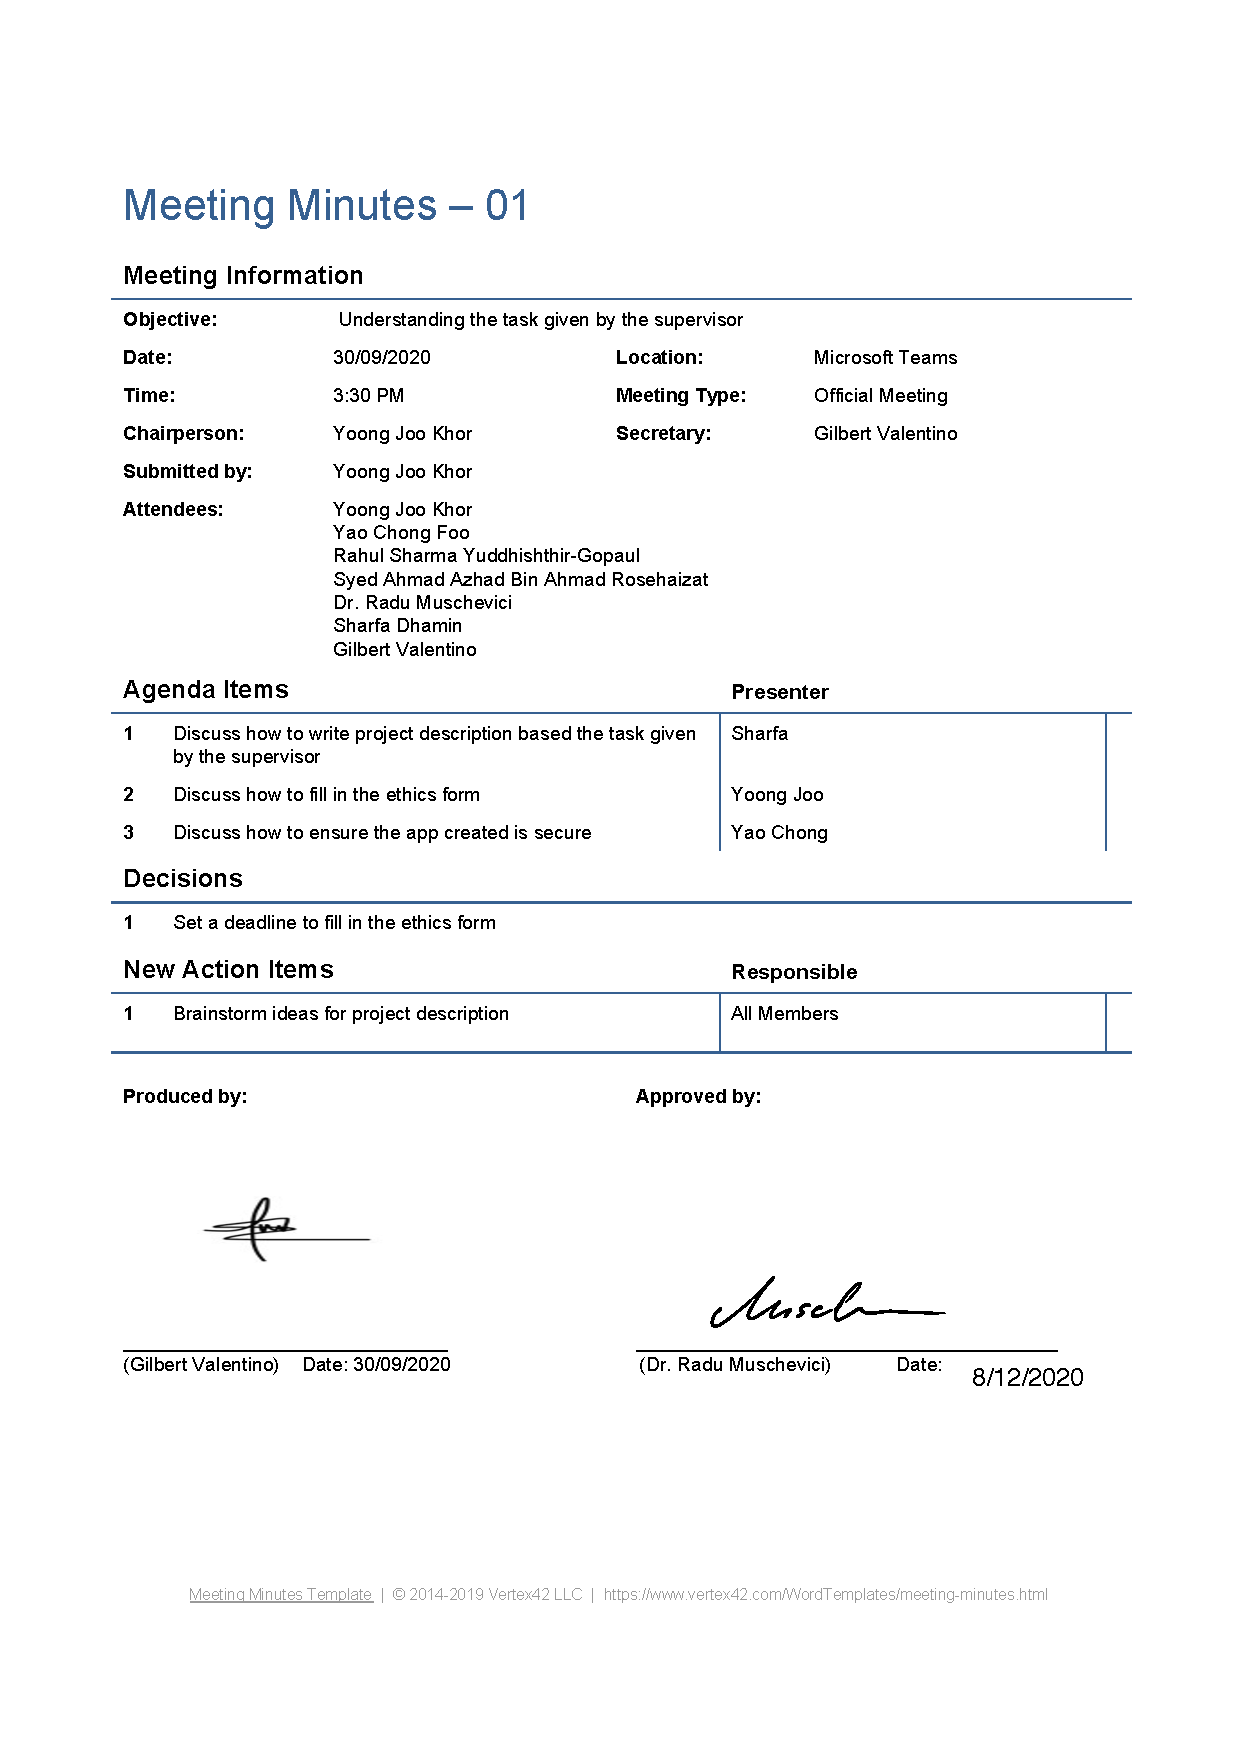
\includepdf[scale=0.95,pagecommand=\section{Meeting Minutes}]{../minutes/Meeting Minutes - 01.pdf}
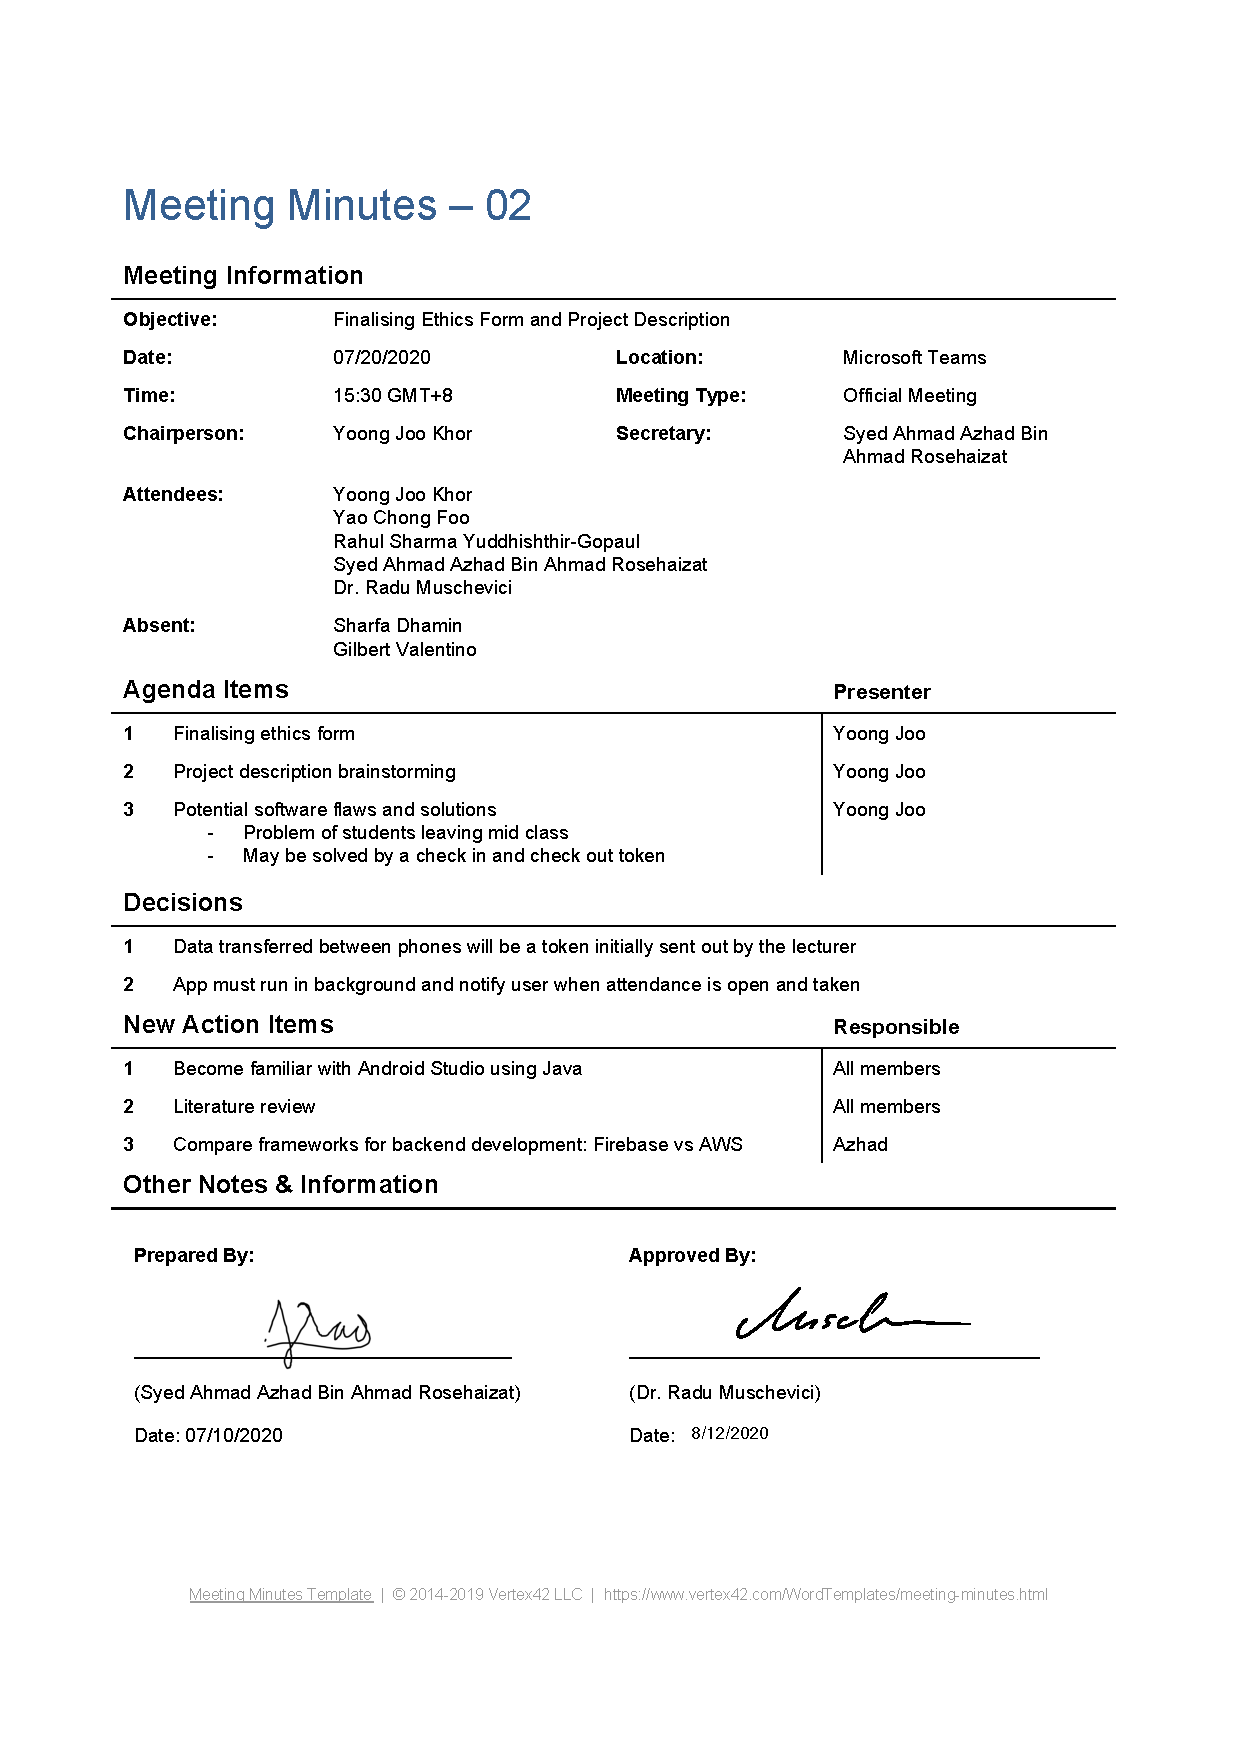
\includepdf[scale=0.95]{../minutes/Meeting Minutes - 02.pdf}
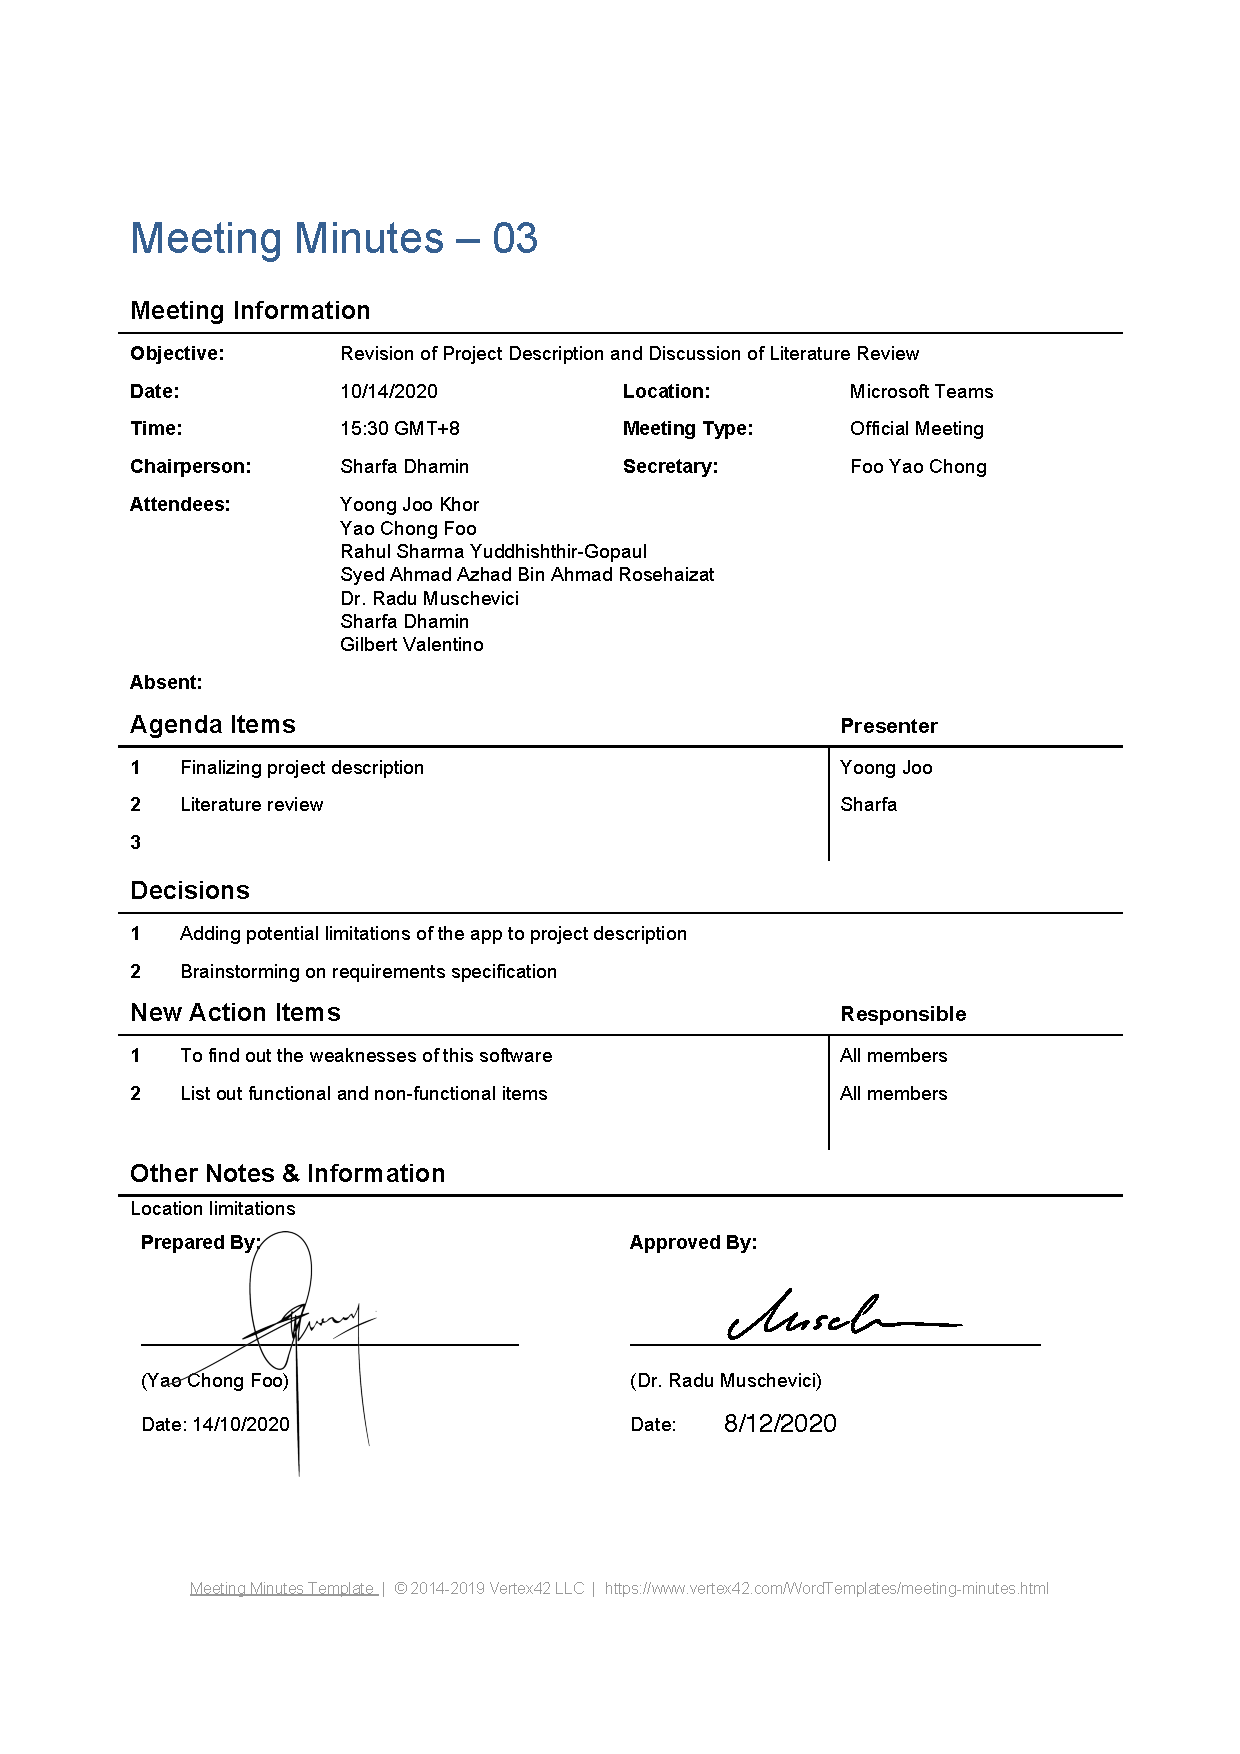
\includepdf[scale=0.95]{../minutes/Meeting Minutes - 03.pdf}
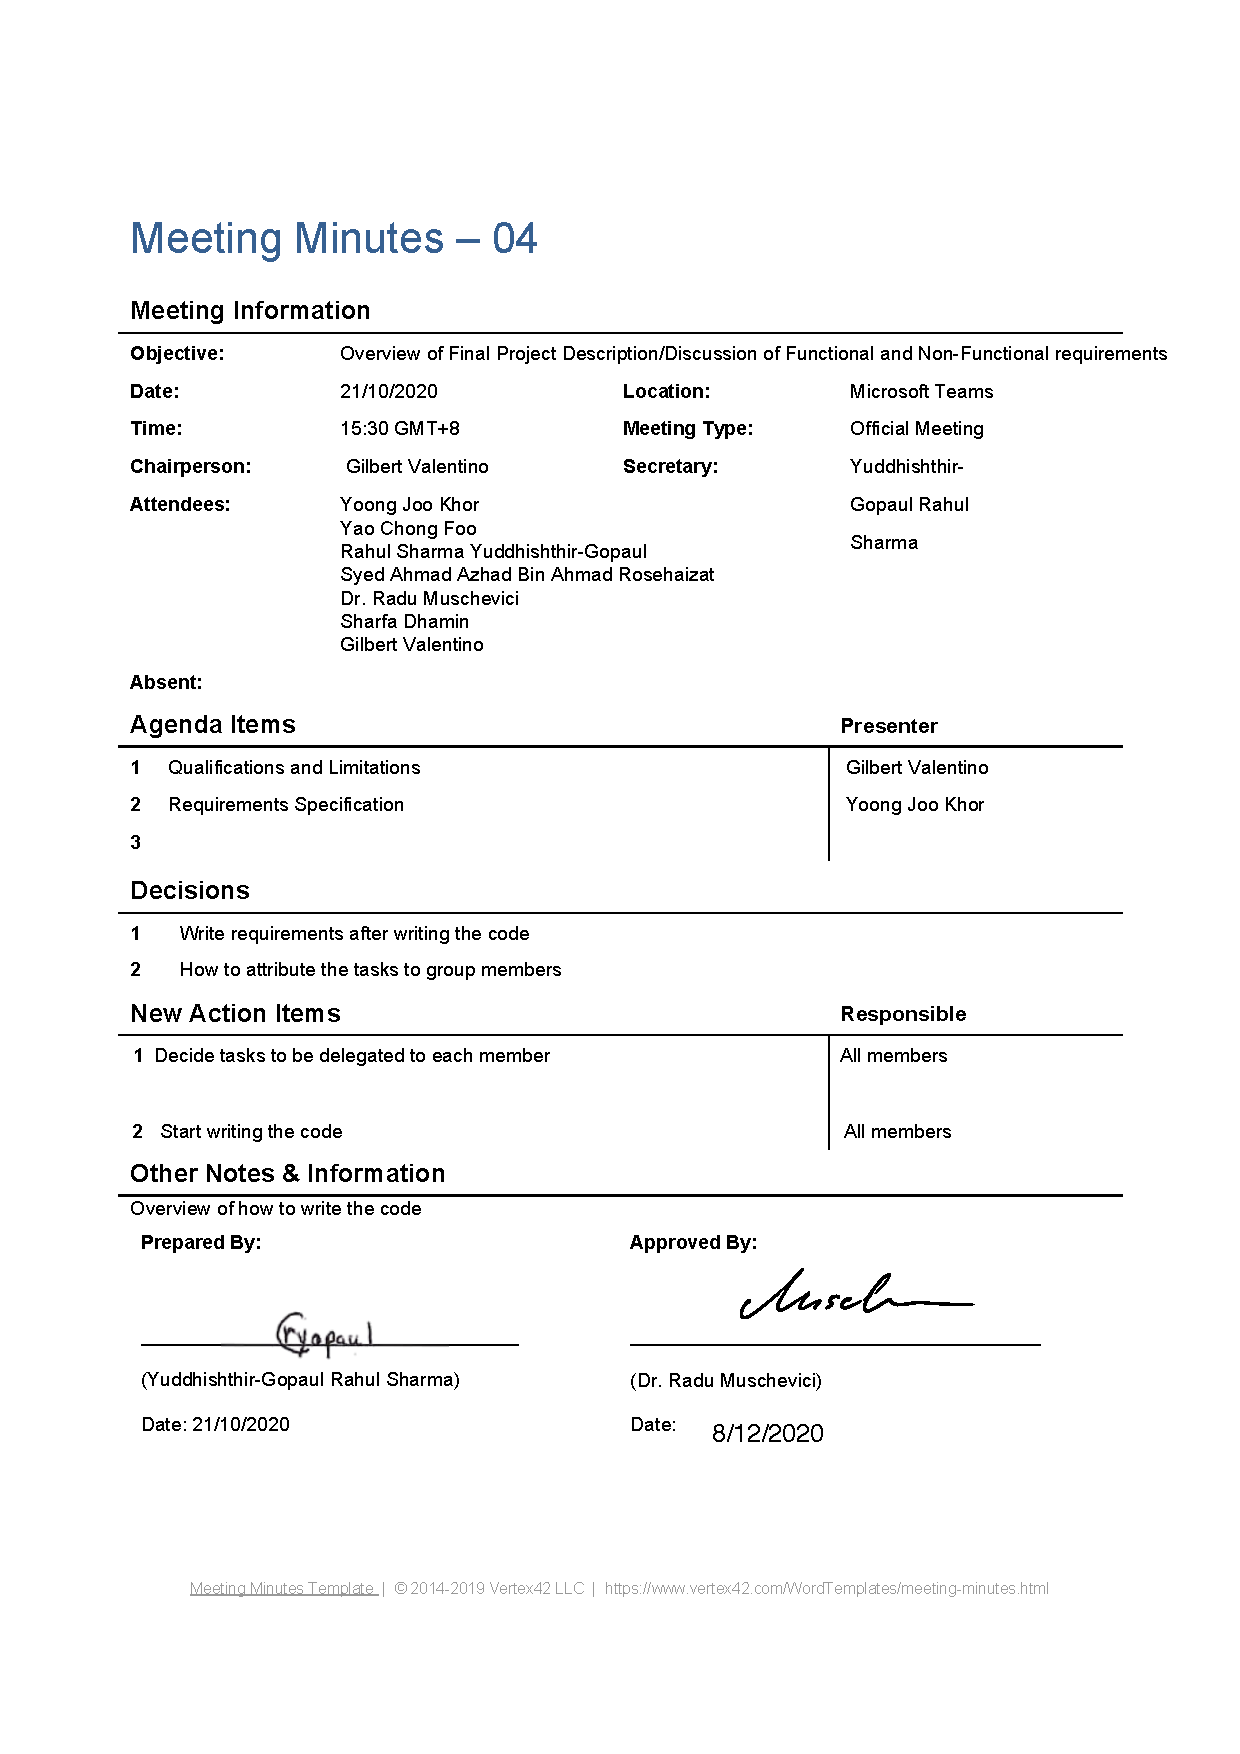
\includepdf[scale=0.95]{../minutes/Meeting Minutes - 04.pdf}
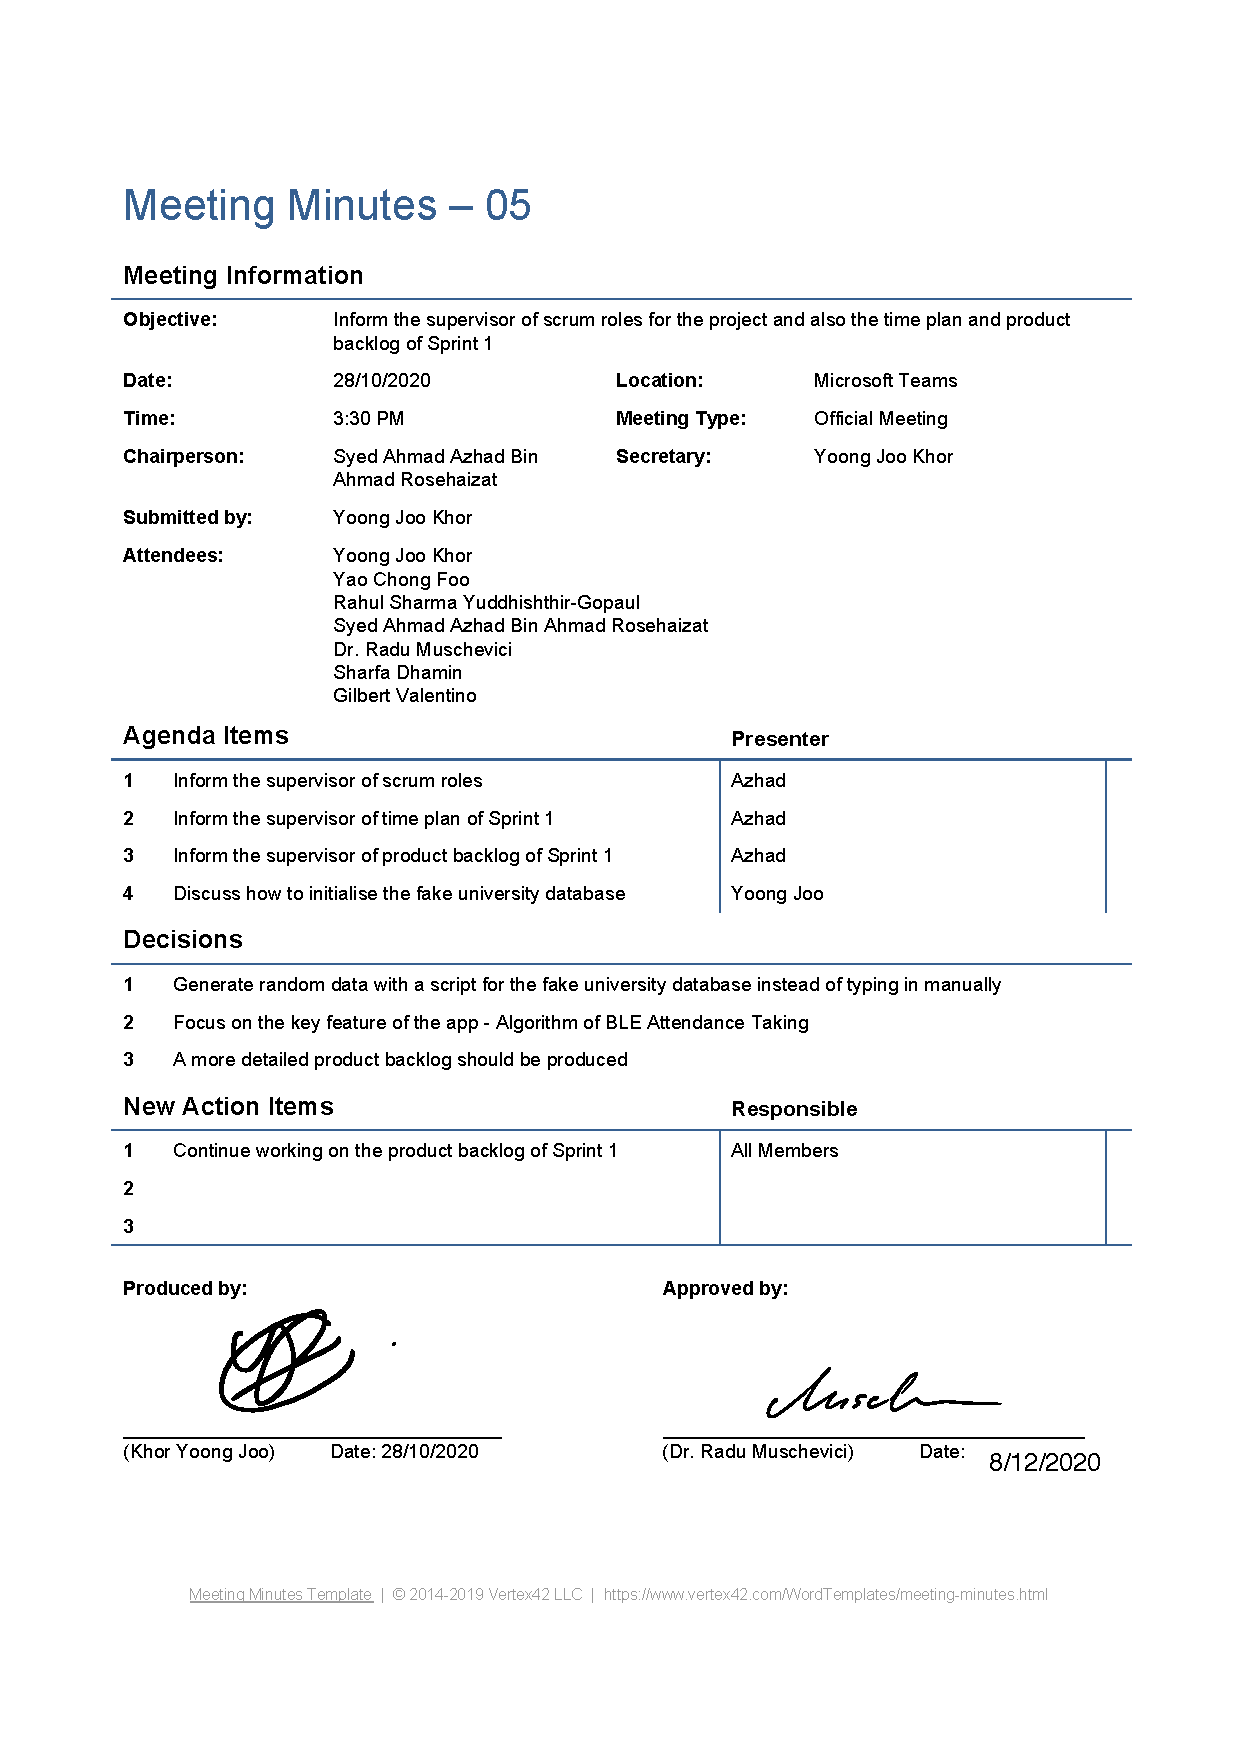
\includepdf[scale=0.95]{../minutes/Meeting Minutes - 05.pdf}
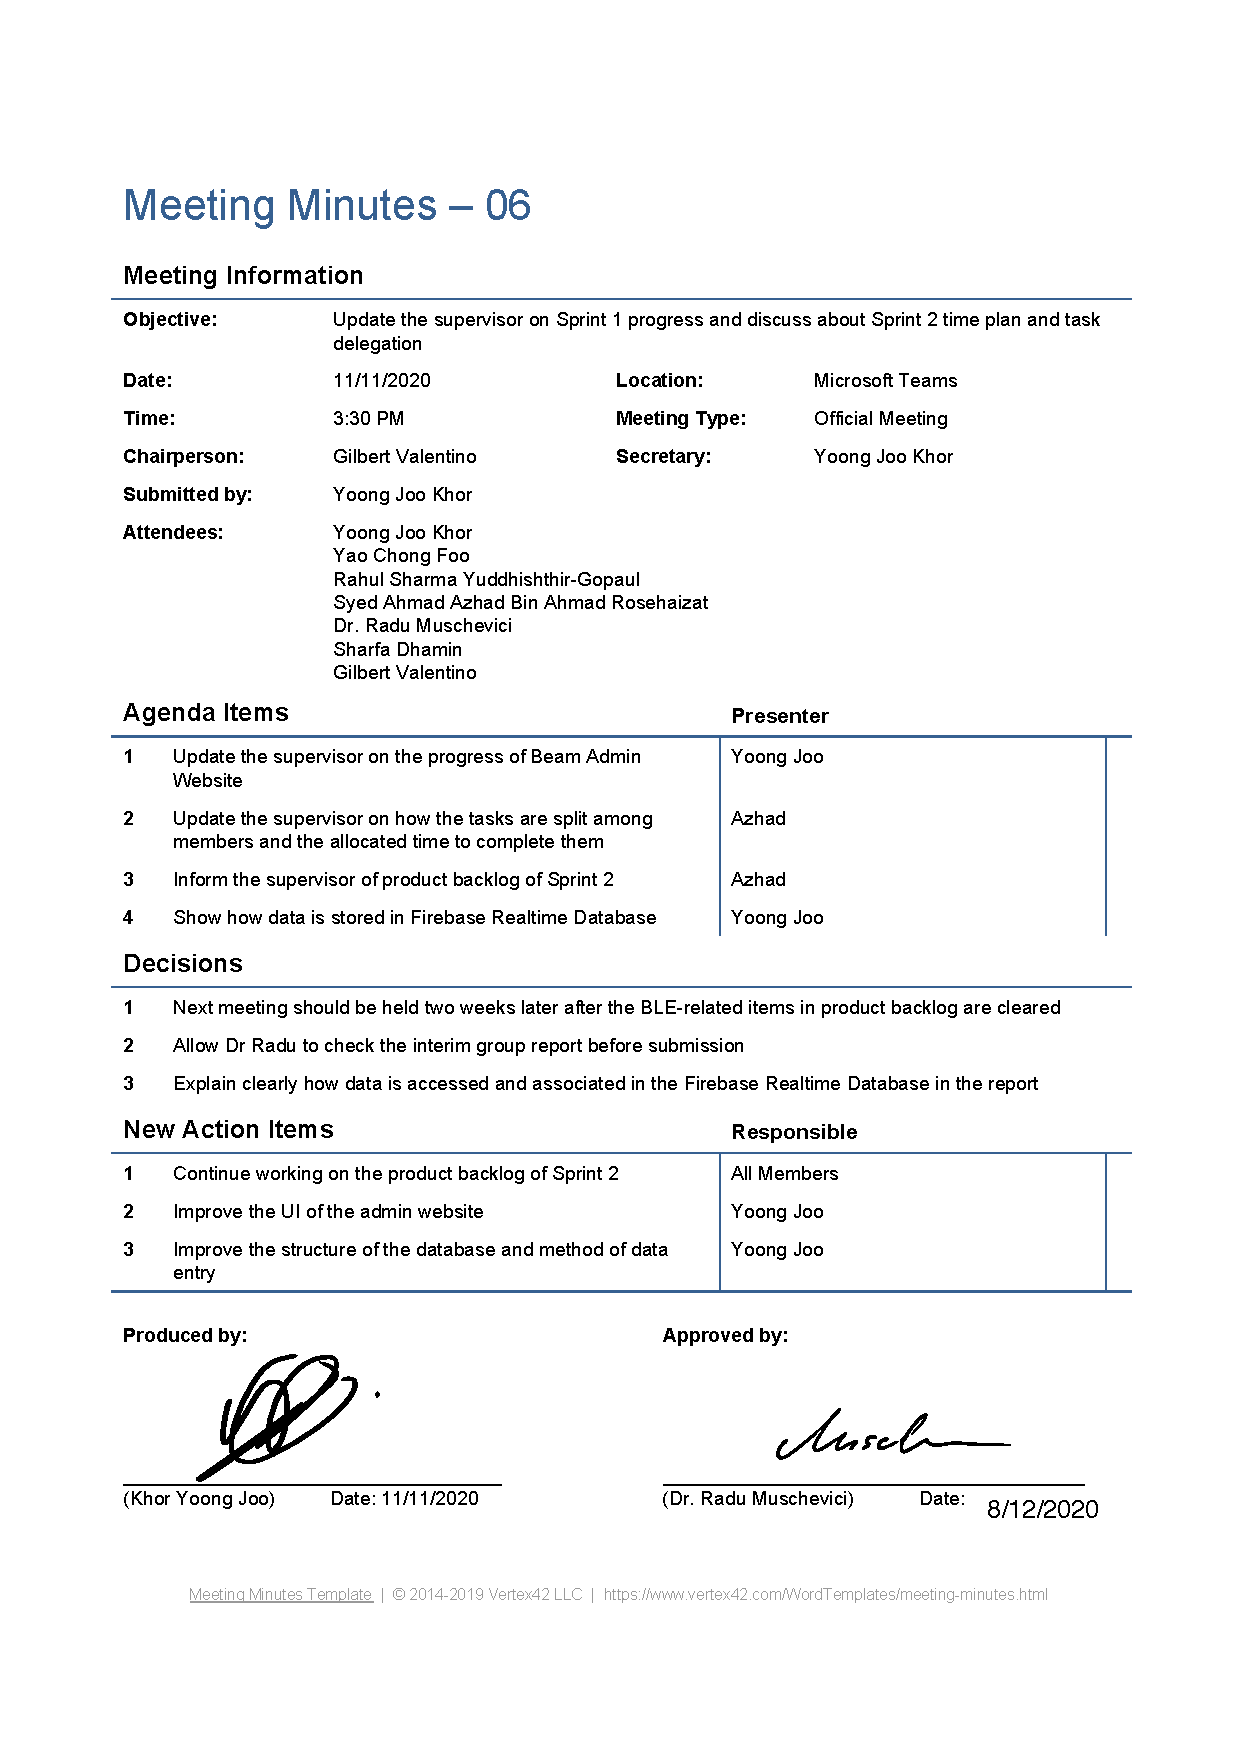
\includepdf[scale=0.95]{../minutes/Meeting Minutes - 06.pdf}
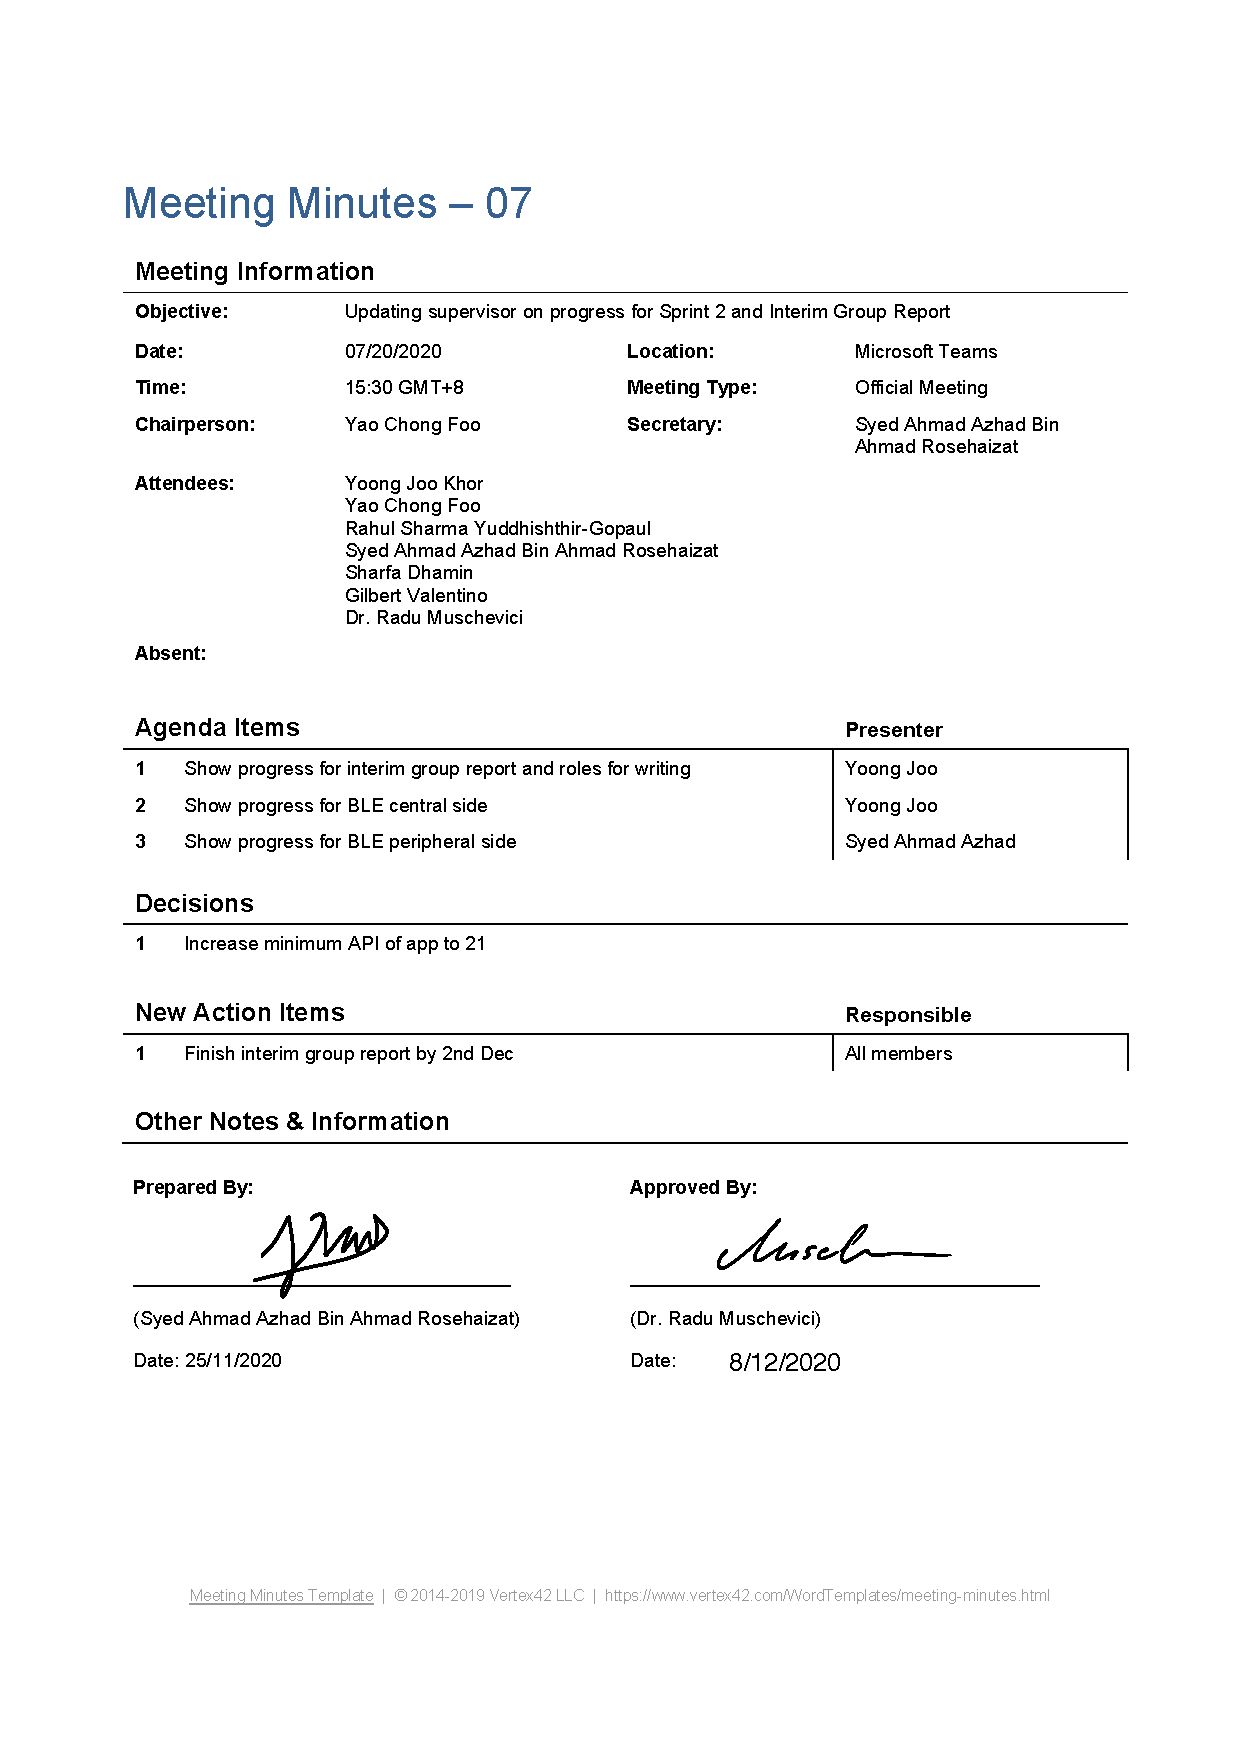
\includepdf[scale=0.95]{../minutes/Meeting Minutes - 07.pdf}
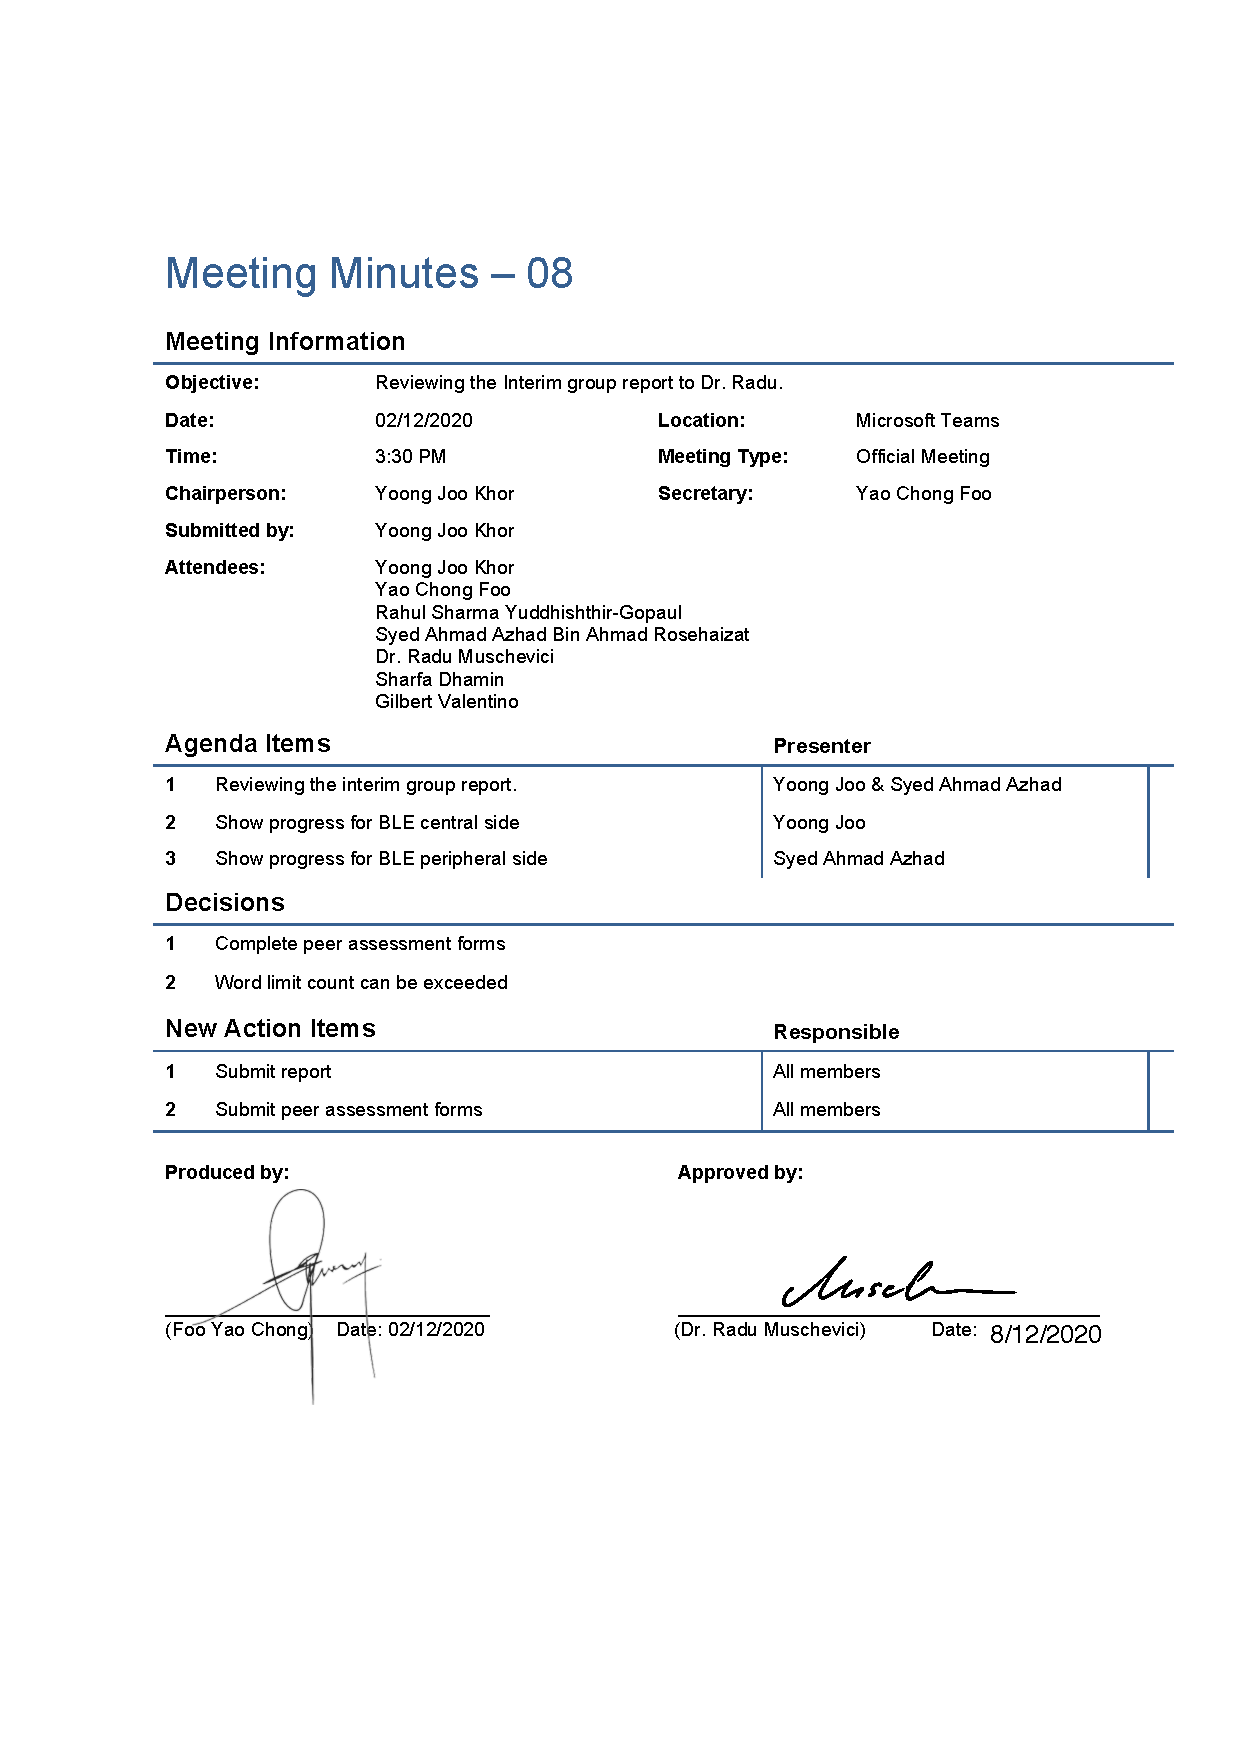
\includepdf[scale=0.95]{../minutes/Meeting Minutes - 08.pdf}
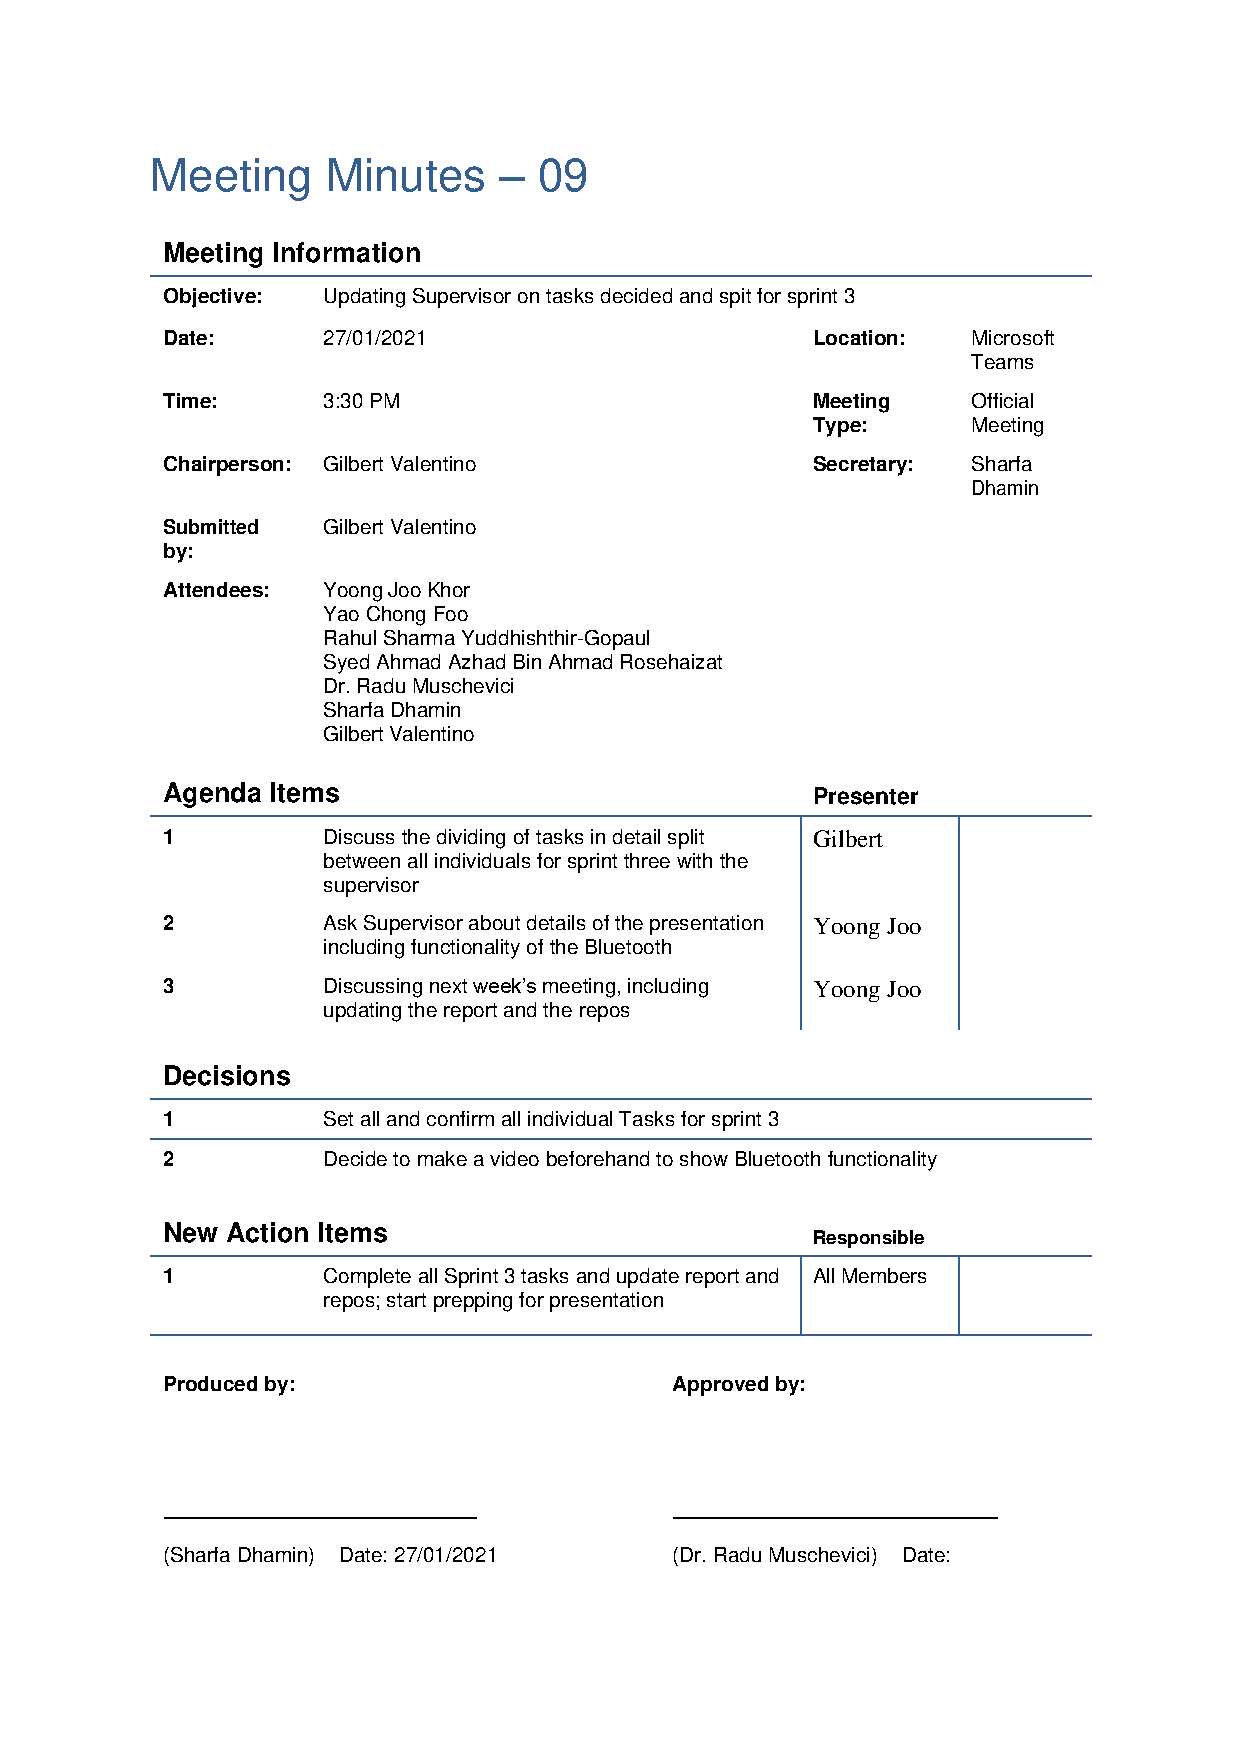
\includepdf[scale=0.95]{../minutes/Meeting Minutes - 09.pdf}
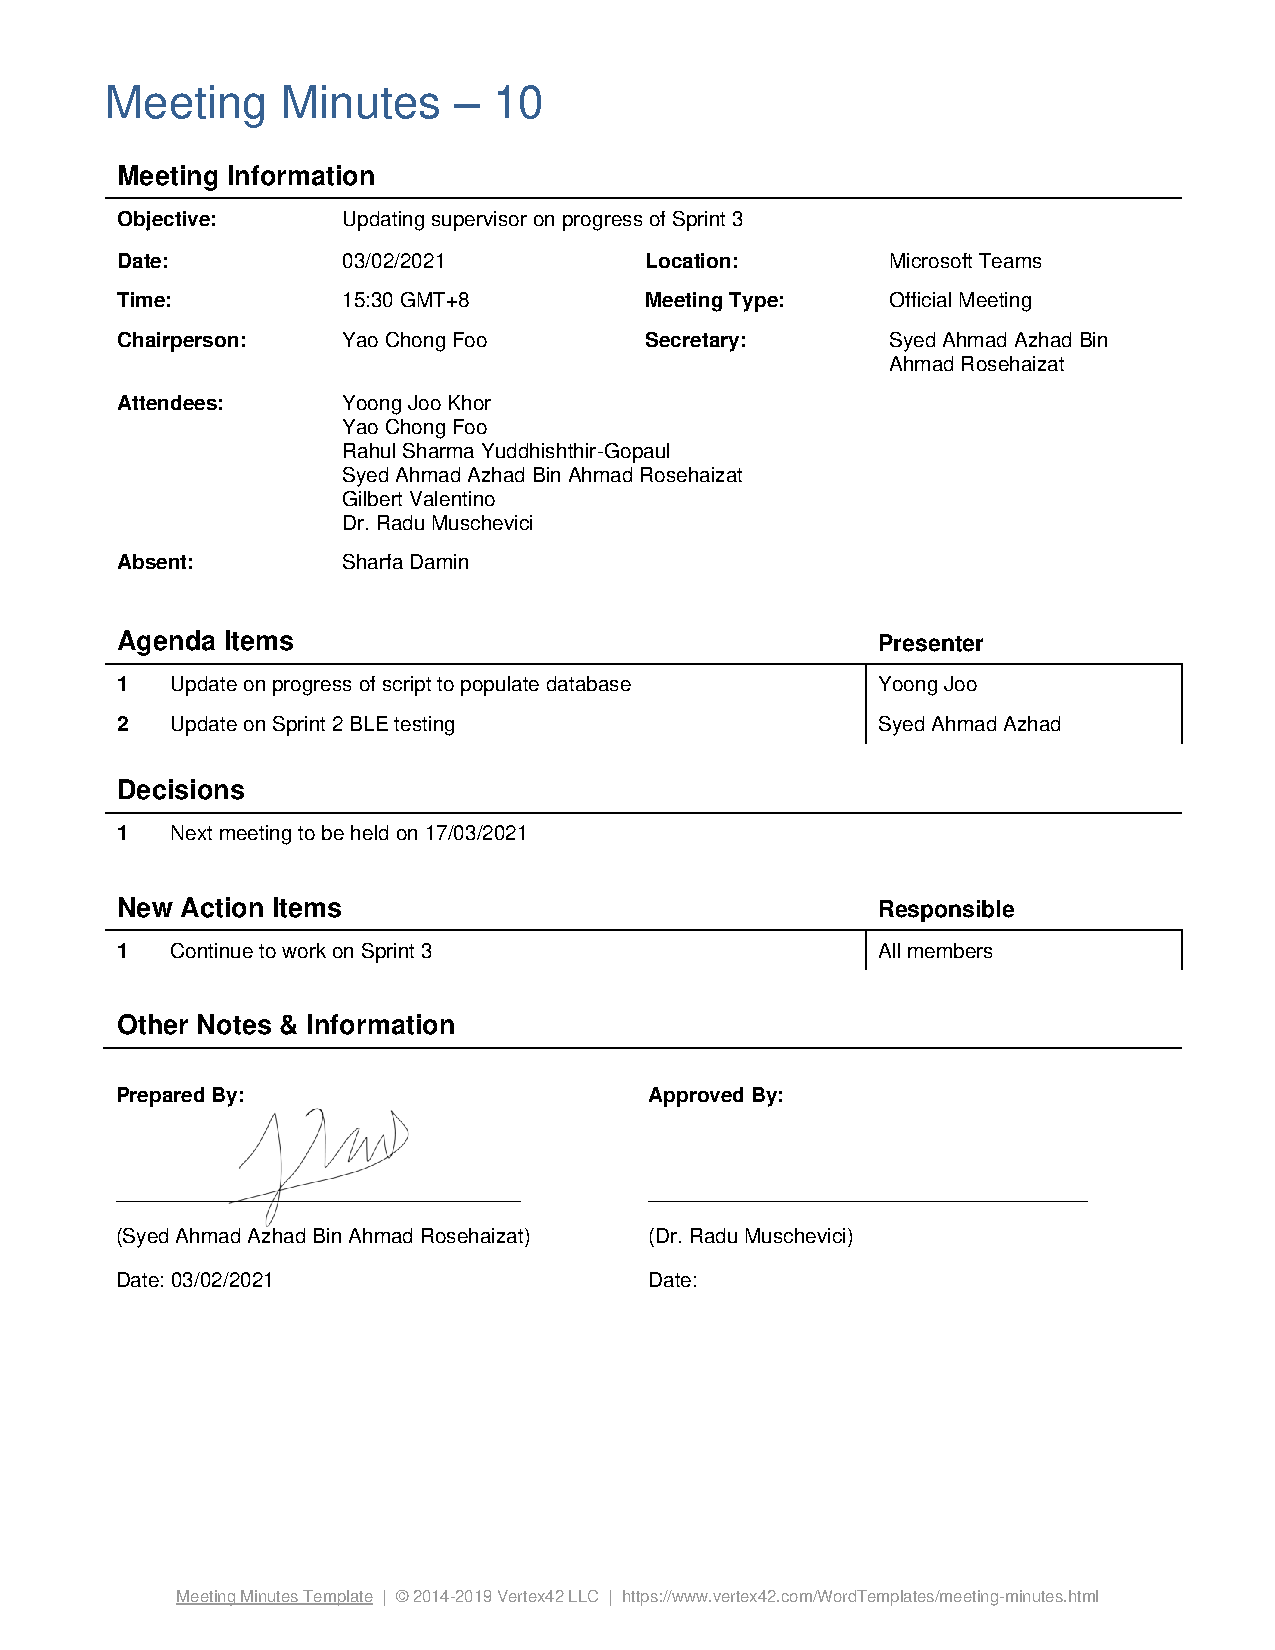
\includepdf[scale=0.95]{../minutes/Meeting Minutes - 10.pdf}
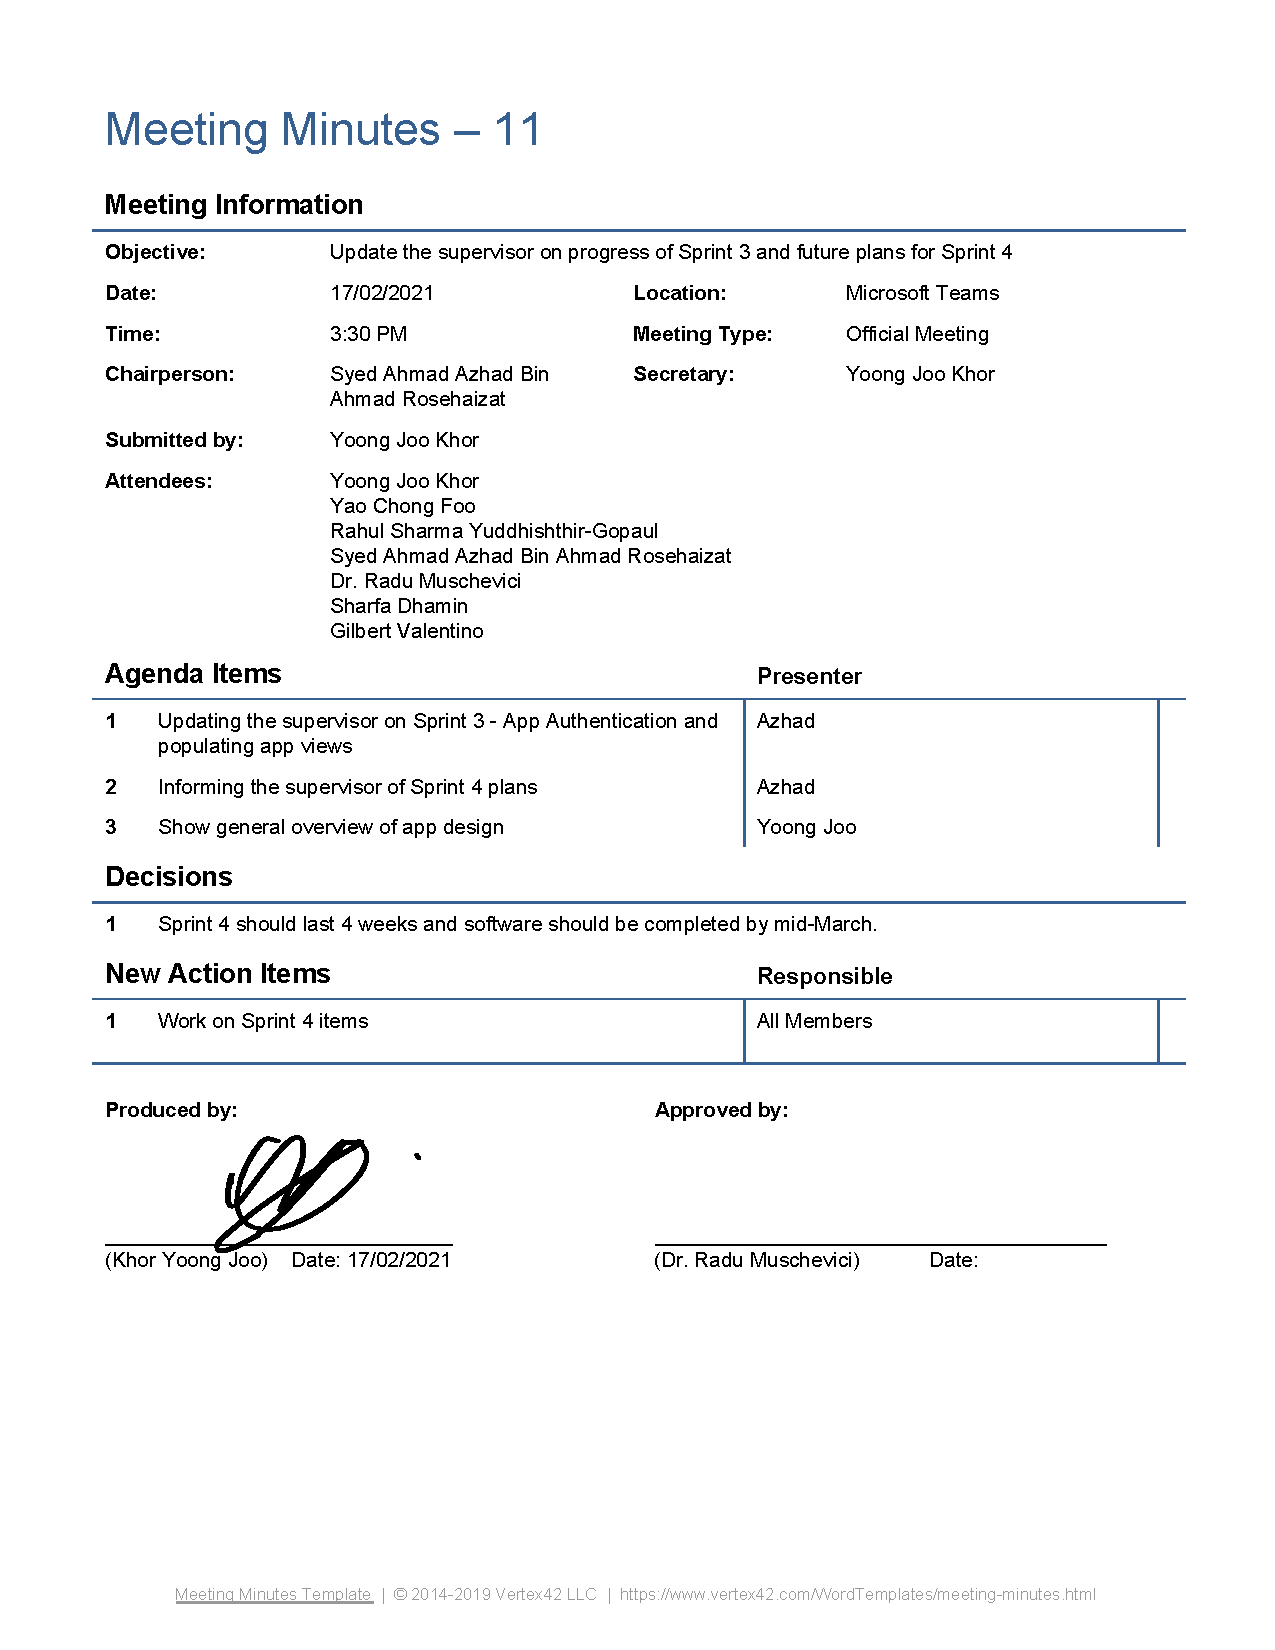
\includepdf[scale=0.95]{../minutes/Meeting Minutes - 11.pdf}
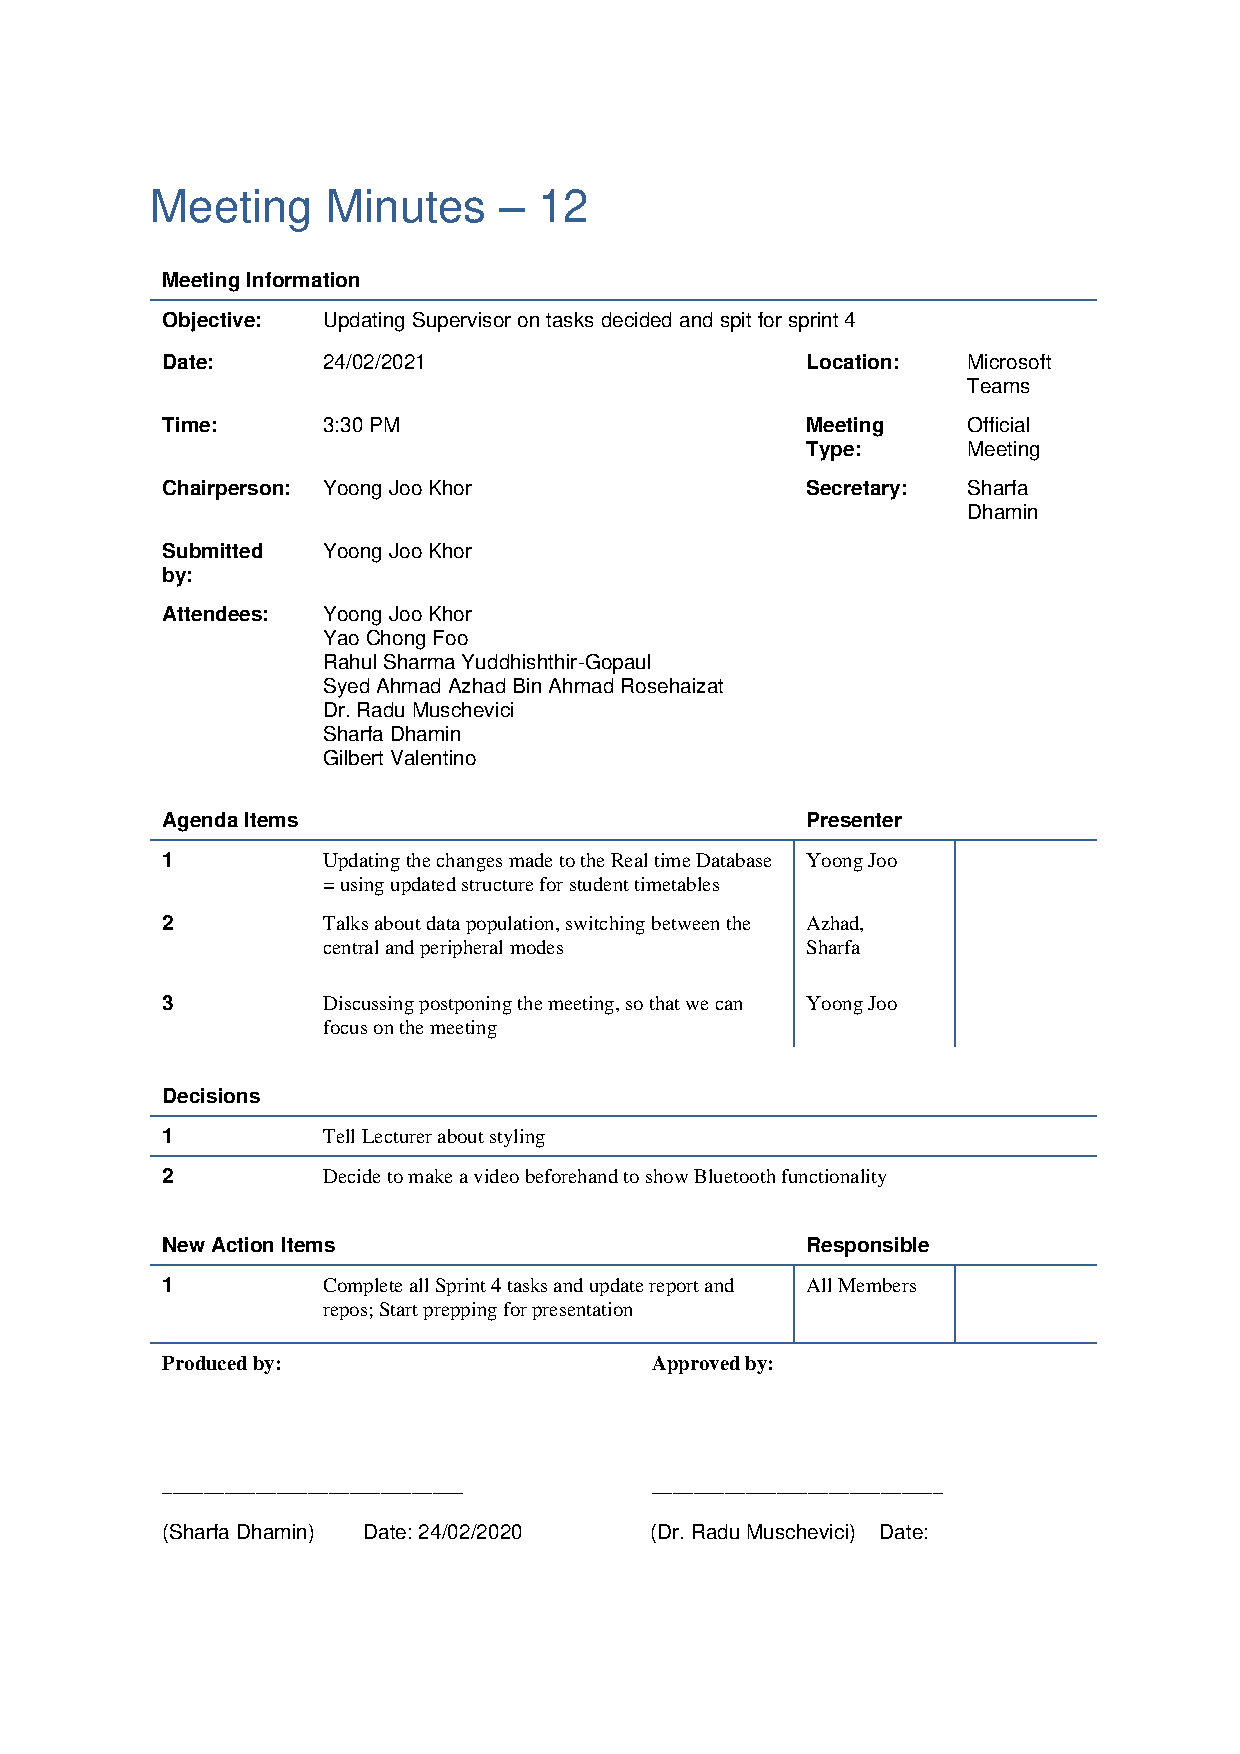
\includepdf[scale=0.95]{../minutes/Meeting Minutes - 12.pdf}
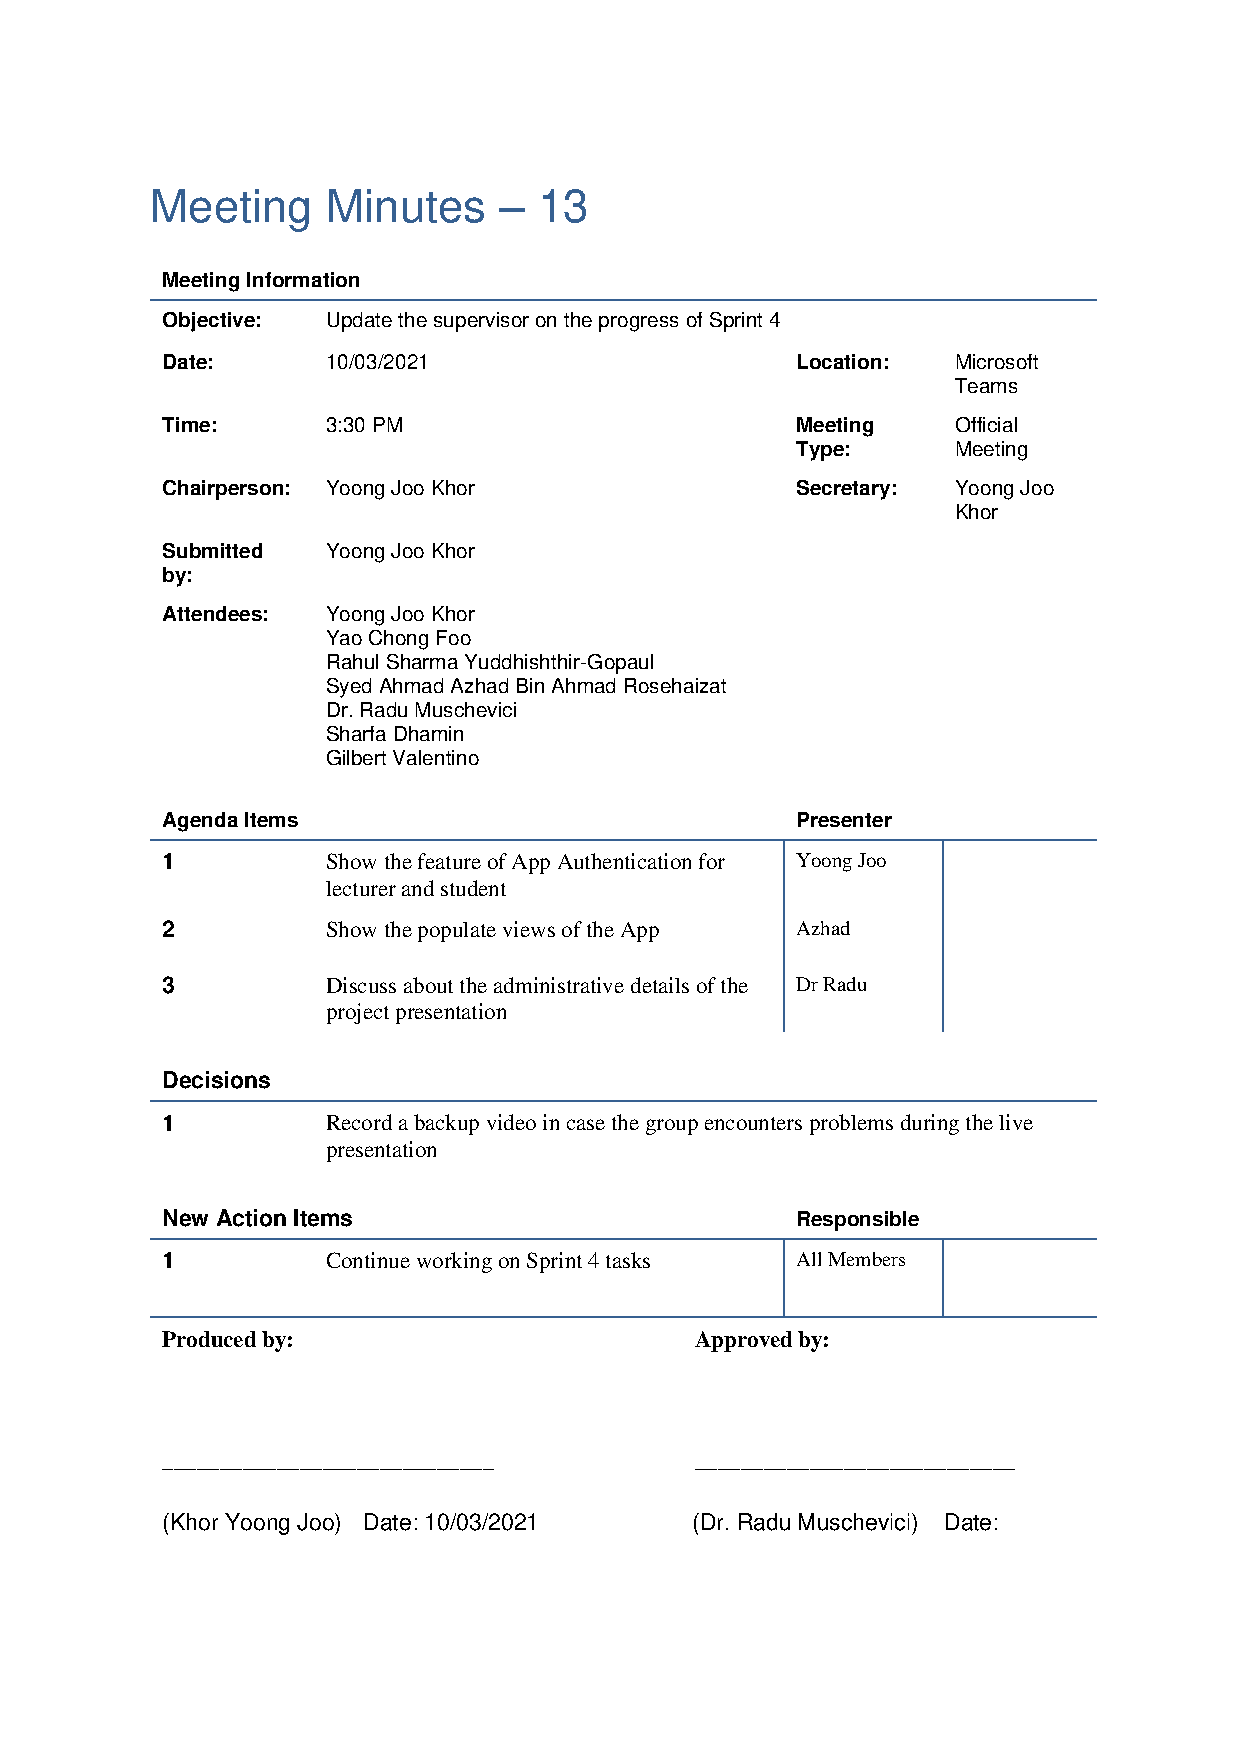
\includepdf[scale=0.95]{../minutes/Meeting Minutes - 13.pdf}
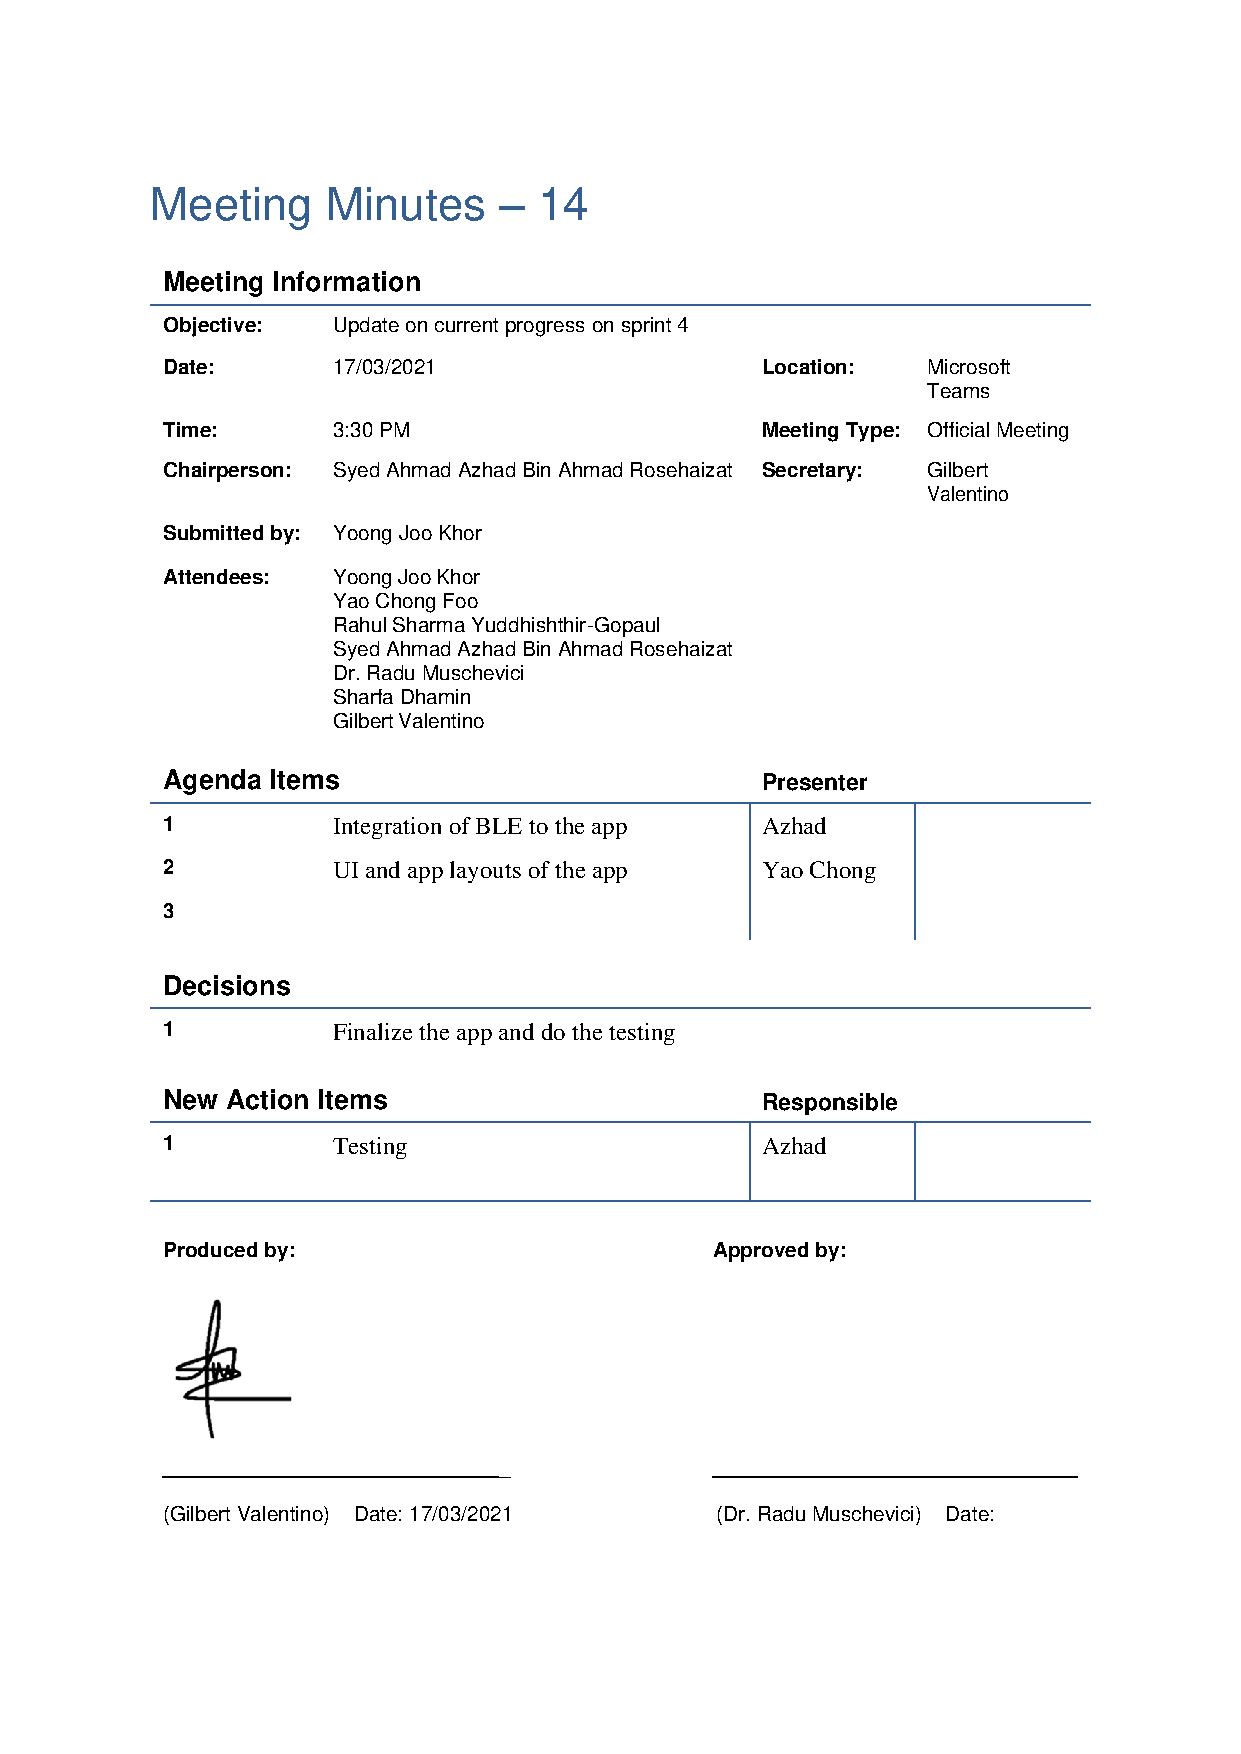
\includepdf[scale=0.95]{../minutes/Meeting Minutes - 14.pdf}
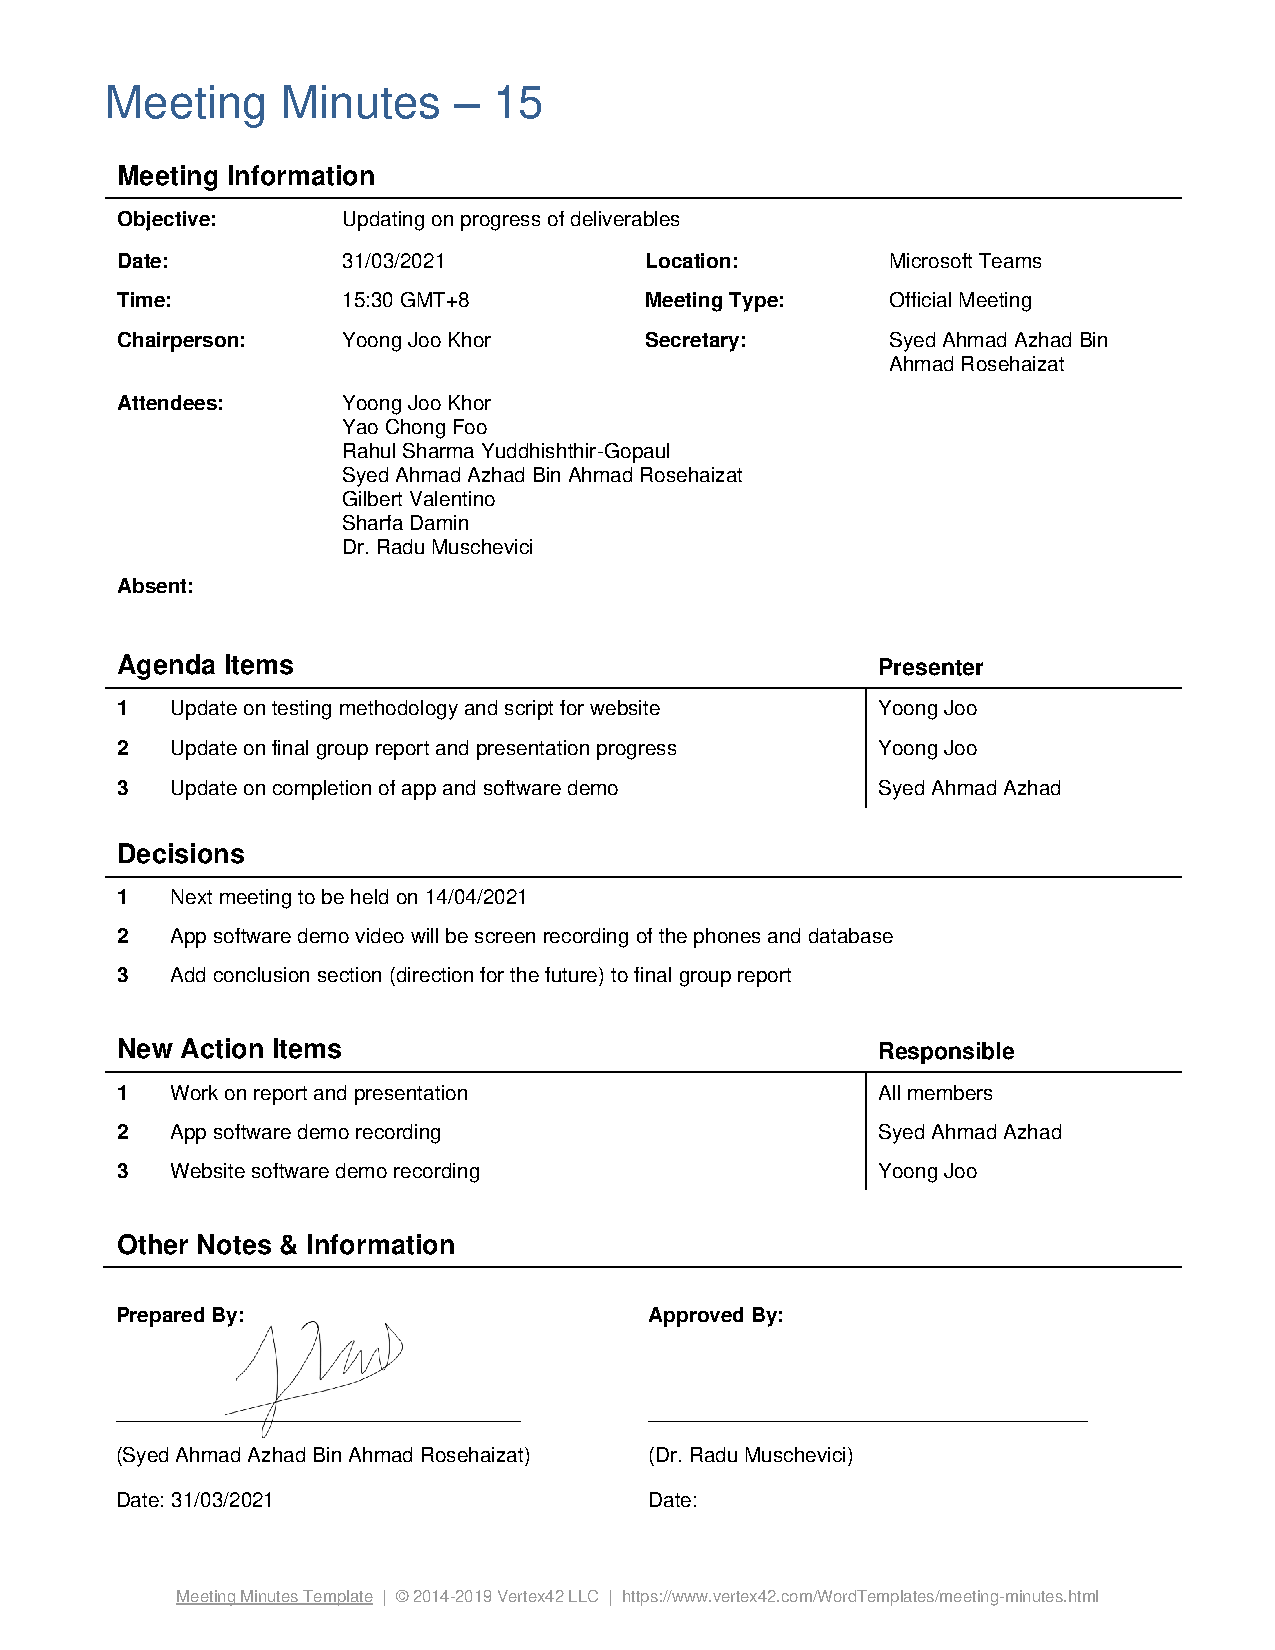
\includepdf[scale=0.95]{../minutes/Meeting Minutes - 15.pdf}
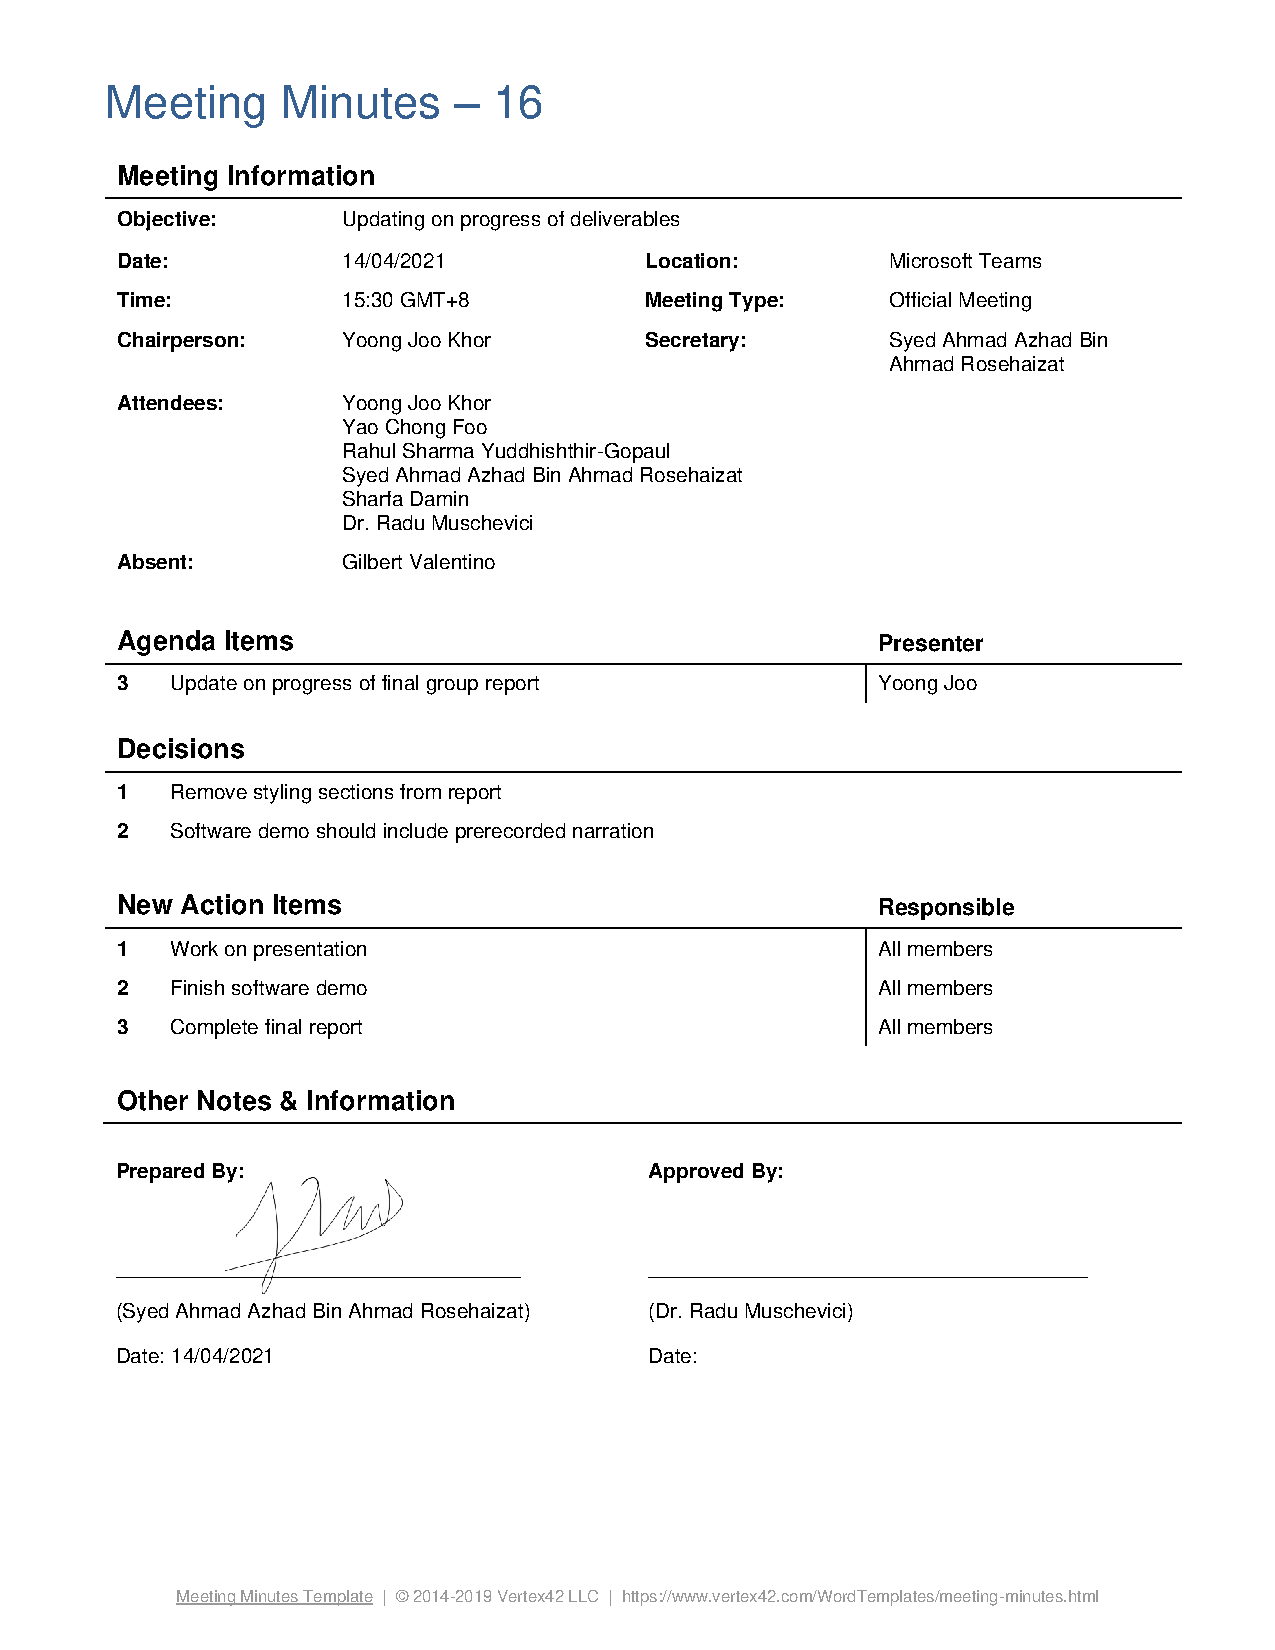
\includepdf[scale=0.95]{../minutes/Meeting Minutes - 16.pdf}
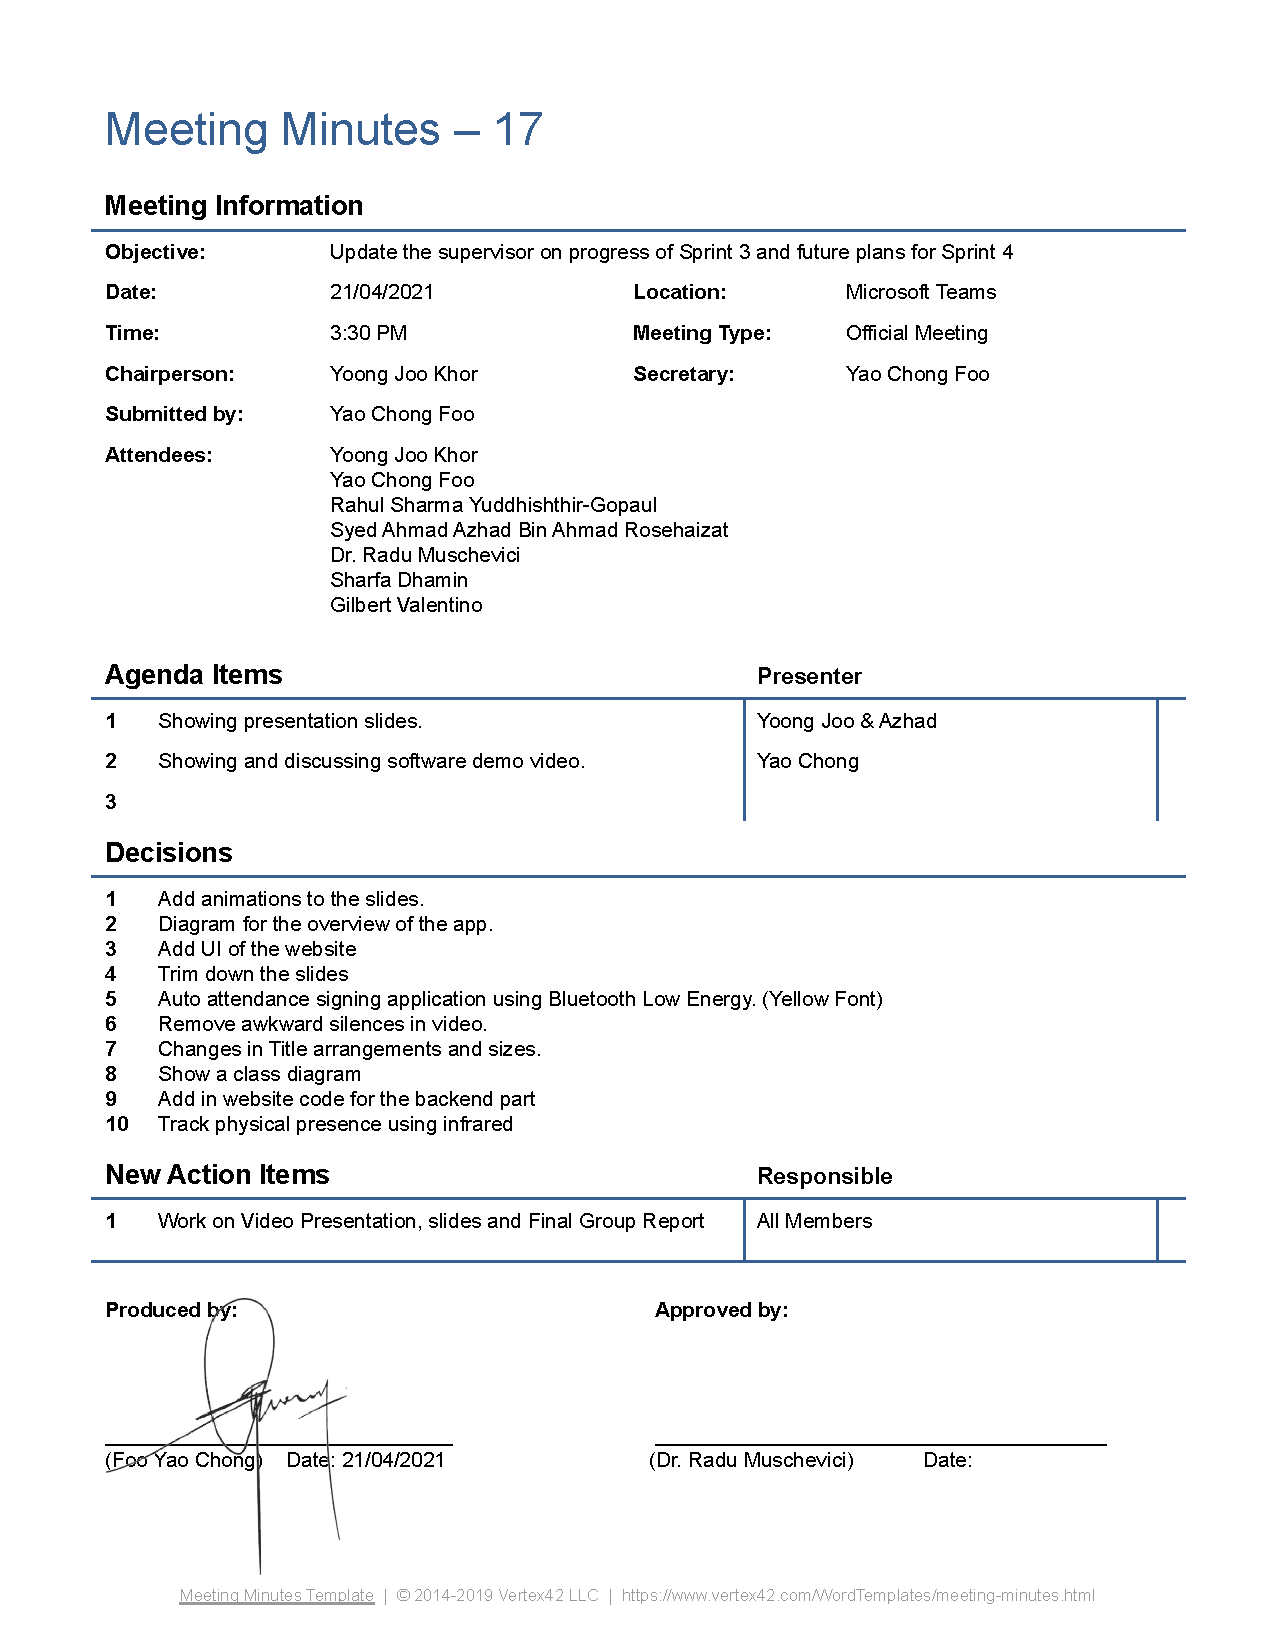
\includepdf[scale=0.95]{../minutes/Meeting Minutes - 17.pdf}
\end{document}